\documentclass[%
reprint,
superscriptaddress,
%groupedaddress,
%unsortedaddress,
%runinaddress,
%frontmatterverbose,
%preprint,
showpacs,preprintnumbers,
%nofootinbib,
%nobibnotes,
%bibnotes,
 amsmath,amssymb,
 aps,
%pra,
%prb,
prd,
%prl,
%rmp,
%prstab,
%prstper,
%floatfix,
]{revtex4-1}

\usepackage{float}
\usepackage{graphicx}% Include figure files
\usepackage{dcolumn}% Align table columns on decimal point
\usepackage{bm}% bold math
\usepackage{bbold}
\usepackage{braket}
\usepackage{amssymb,amsmath}
\usepackage{hyperref}% add hypertext capabilities
%\usepackage[mathlines]{lineno}% Enable numbering of text and display math
%\linenumbers\relax % Commence numbering lines

%\usepackage[showframe,%Uncomment any one of the following lines to test
%%scale=0.7, marginratio={1:1, 2:3}, ignoreall,% default settings
%%text={7in,10in},centering,
%%margin=1.5in,
%%total={6.5in,8.75in}, top=1.2in, left=0.9in, includefoot,
%%height=10in,a5paper,hmargin={3cm,0.8in},
%]{geometry}



\usepackage{color}
\usepackage[dvipsnames, svgnames, x11names]{xcolor}
\usepackage{amsfonts}
\usepackage{subfigure}
\usepackage{array}


\newcommand{\Tr}{\ensuremath{\operatorname{Tr}}}
\newcommand{\tr}{\ensuremath{\operatorname{tr}}}
\newcommand{\Omegaqq}{\ensuremath{\Omega_{\bar{q}q}}}
\newcommand{\vev}[1]{\ensuremath{\left\langle #1 \right\rangle}}
\newcommand{\einh}[1]{\ensuremath{\,\text{#1}}}
\newcolumntype{L}{>{\centering\arraybackslash}m{3cm}}



\newcommand{\overbar}[1]{\mkern 1.5mu\overline{\mkern-1.5mu#1\mkern-1.5mu}\mkern 1.5mu}

\definecolor{bjcol}{rgb}{1,.44,0.13}

% color def's

\definecolor{blue}{rgb}{0,0,1}
\newcommand{\colb}[1]{{\color{blue} #1}}
\definecolor{green}{rgb}{0,1,0}
\newcommand{\colg}[1]{{\color{green} #1}}
\definecolor{red}{rgb}{1,0,0}
\newcommand{\colr}[1]{{\color{red} #1}}
\newcommand{\colJ}[1]{{\color{cyan} #1}}
\definecolor{gray}{rgb}{.5,.5,.5}
\newcommand{\drop}[1]{{\sout{ {\color{gray} #1}}}}
\definecolor{darkgreen}{rgb}{.0,.5,.0}
\newcommand{\colL}[1]{{\color{darkgreen} #1}}


\def\Fig#1{Fig.~\ref{#1}} \def\Tab#1{Tab.~\ref{#1}}
\def\Figs#1{Figs.~\ref{#1}} \def\Tab#1{Tab.~\ref{#1}}
\def\Eqs#1{Eqs.~(\ref{#1})}
\def\Eq#1{Eq.~(\ref{#1})}
\def\eq#1{(\ref{#1})}
\def\eqref#1{(\ref{#1})}
\def\fig#1{Fig.~\ref{#1}}
\def\tab#1{Tab.~\ref{#1}}
\def\eqs#1{(\ref{#1})}
\def\Eqs#1{(\ref{#1})}
\def\sec#1{Sec.~\ref{#1}}
\def\app#1{Appendix~\ref{#1}}
\newcommand{\Phibar}{\ensuremath{\bar{\Phi}}}
\newcommand{\LPQM}{\ensuremath{\mathcal{L}_{\textrm{PQM}}}\xspace}

\def\dbar{{\mathchar'26\mkern-12mu d}}
\def\lA0{{\langle A_0 \rangle}}
\def\bA0{{\bar{A}_0}}
\def\lLA{{\langle L[A_0] \rangle}}
\def\lL{{\langle L \rangle}}
\def\lLc{{\langle L^\dagger \rangle}}
\def\lLAc{{\langle L^\dagger[A_0] \rangle}}


\def\dr{{D\!\llap{/}}\,}
\def\Dr{{D\!\llap{/}}\,}
\def\ipv{\vec{p}\llap{/}}
\def\pslash{p\llap{/}}

\def\0#1#2{\frac{#1}{#2}}

\newcommand{\bsig}{\ensuremath{\bar{\sigma}}}
\newcommand{\lsm}{L\ensuremath{\sigma}M\xspace}
\newcommand{\pT}{\ensuremath{T_0}}
\newcommand{\Tl}{\ensuremath{T_\chi}}
\newcommand{\Ts}{\ensuremath{T_\chi^s}}
\newcommand{\Tchi}{\ensuremath{T_\chi}}
\newcommand{\Td}{\ensuremath{T_d}}
\newcommand{\Tc}{\ensuremath{T_c}}
\newcommand{\muc}{\ensuremath{\mu_c}}
\newcommand{\coloronl}{(color online)\xspace}

\newcommand{\mrm}[1]{\mathrm{#1}}
\def\qbar{\bar{q}}
\newcommand{\sx}{\sigma_{x}}
\newcommand{\sy}{\sigma_{y}}

%%%%%%%%%%%%%% for corrections %%%%%%%%%%%
\newcommand{\colwj}[1]{\textcolor{Purple}{#1}}
\newcommand{\colxf}[1]{\textcolor{cyan}{#1}}
\newcommand{\coljan}[1]{\textcolor{red}{#1}}
\newcommand{\colfab}[1]{\textcolor{magenta}{#1}}
\newcommand{\colrui}[1]{\textcolor{green}{#1}}
\newcommand{\colnu}[1]{\textcolor{blue}{#1}}
\newcommand{\colshi}[1]{\textcolor{Plum}{#1}}

%
%%%%%%%%%%%%%%%%%%%%%%%%%%%%%%%%%%%%%%%%%%%%%%%%%%%%%%%%%%%%%%%%%%%%%%%%%%%%%

\graphicspath{{./figures/}{./}}

\begin{document}

\preprint{}

\title{Hyper-order baryon number fluctuations at finite temperature and density}



\affiliation{Key Laboratory of Quark \& Lepton Physics (MOE) and Institute of Particle Physics,
Central China Normal University, Wuhan 430079, China}

\author{Wei-jie Fu}
\affiliation{School of Physics, Dalian University of Technology, Dalian, 116024,
  P.R. China}

\author{Xiaofeng Luo}
\affiliation{Key Laboratory of Quark \& Lepton Physics (MOE) and Institute of Particle Physics,
Central China Normal University, Wuhan 430079, China}

\author{Jan M. Pawlowski}
\affiliation{Institut f\"ur Theoretische Physik, Universit\"at Heidelberg, Philosophenweg 16, 69120 Heidelberg, Germany}
\affiliation{ExtreMe Matter Institute EMMI, GSI, Planckstra{\ss}e 1, D-64291 Darmstadt, Germany}

\author{Fabian Rennecke}
\affiliation{Physics Department, Brookhaven National Laboratory, Upton, NY 11973, USA}

\author{Rui Wen}
\affiliation{School of Physics, Dalian University of Technology, Dalian, 116024,
  P.R. China}

\author{Shi Yin}
\affiliation{School of Physics, Dalian University of Technology, Dalian, 116024,
  P.R. China}


%\date{\today}% It is always \today, today,
             %  but any date may be explicitly specified

\begin{abstract}

We study the fourth- to tenth order (hyper-order) baryon number fluctuations at finite temperature and density in an advanced (QCD-assisted) low energy effective theory that includes low energy quantum, thermal and density fluctuations. At vanishing density our results agree quantitatively, both with lattice QCD simulations for temperatures $T\gtrsim 140$\, MeV, and with the hadron resonance gas for $T\lesssim 120$\,MeV. Furthermore, we compute the dependence of the baryon number fluctuations on the collision energy, which is compared with recent experimental measurements of the kurtosis and the sixth-order cumulant of the net-proton distribution from the STAR collaboration. 

The current approach shows a non-monotonic behavior of higher order cumulants as a function of the beam-energy measured by STAR. In the respective regime the QCD-assisted low energy effective theory used shows no critical behaviour. This asks for a refined analysis of hyper fluctuations within first principles QCD, whose setup is also discussed here.  

\end{abstract}
%\pacs{Valid PACS appear here}% PACS, the Physics and Astronomy
\pacs{11.30.Rd, %Chiral symmetries
         11.10.Wx, %Finite-temperature field theory
         05.10.Cc, %Renormalization group methods
         12.38.Mh  %Quark-gluon plasma
     }                             % Classification Scheme.
%\keywords{Suggested keywords}%Use showkeys class option if keyword
                              %display desired
\maketitle
%\tableofcontents

%%%%%%%%%%%%%%%%%%%%%%%%%%%%%%%%%%%%%%%%%%%%%%%%%%%%%%%%%%%
%%%%%%%%%%%%%%%%%%%%%%%%%%%%%%%%%%%%%%%%%%%%%%%%%%%%%%%%%%%

\section{Introduction}
\label{sec:int}

Lots of effort have been made to study the QCD phase structure at finite temperature and density over the last few decades, both from the experimental and theoretical sides \cite{Luo:2017faz,Bzdak:2019pkr,Fischer:2018sdj,Fu:2019hdw}. One of the most intriguing open questions concerning the QCD phase diagram is the existence of the critical end point (CEP) \cite{Stephanov:2007fk}, which is assumed to be located at the end of the first-order phase transition line in the $T-\mu_B$ phase diagram. Here $T$ and $\mu_B$ are referred to the temperature and baryon chemical potential, respectively. In view of the uniqueness and importance of CEP, pinning down its location has played a pivotal role in understanding phases of strongly interacting nuclear matter under extreme conditions. Note that the phase transition at CEP is of genuine second order, and thus the correlation length $\xi$ diverges at this point in the thermodynamic limit. Consequently, critical observables, such as fluctuations of conserved charges that receive contributions in powers of $\xi$ from critical dynamics in the proximity of CEP \cite{Stephanov:2008qz}, are employed to explore the location of CEP \cite{Luo:2017faz,Adam:2020unf}.

Within the Beam Energy Scan (BES) Program at the Relativistic Heavy Ion Collider (RHIC), significant fluctuation measurements have been performed in Phase I, involving the skewness and kurtosis of the net-proton, net-charge, net-kaon multiplicity distributions \cite{Adamczyk:2013dal,Adamczyk:2014fia,Luo:2015ewa,Adamczyk:2017wsl}, second-order off-diagonal cumulants, i.e., correlations of net-proton, net-charge, net-kaon multiplicity distributions \cite{Adam:2019xmk}. Remarkably, very recently the STAR collaboration has reported the first evidence of a non-monotonic variation in kurtosis $\times$ variance of the net-proton number distribution as a function of the collision energy with $3.0\sigma$ significance for central collisions \cite{Adam:2020unf}. Moreover, the measurement has also been extended to the sixth-order cumulant of net-proton and net-charge distributions, and preliminary results have been obtained \cite{Nonaka:2020crv,Pandav:2020uzx}.

The study of fluctuations of conserved charges, e.g., the baryon number, electric charge and the strangeness, has always been an active area of theoretical research. Significant progress in this direction has been made within the lattice QCD simulations \cite{Bazavov:2012vg,Borsanyi:2013hza,Borsanyi:2014ewa,Bazavov:2017dus,Bazavov:2017tot,Borsanyi:2018grb,Bazavov:2020bjn}, in particular in the regime of high $T$ and low $\mu_B$ in the phase diagram. It is, however, difficult to extend lattice simulations to high-$\mu_B$ region due to the sign problem. Remarkably, recent first-principle QCD calculations at finite temperature and density, within both the functional renormalization group (fRG) and Dyson-Schwinger equations (DSE), indicate that the location of CEP is presumably in a region of $450\,\mathrm{MeV} \lesssim\mu_B\lesssim 650\,\mathrm{MeV}$ \cite{Fischer:2018sdj,Fu:2019hdw,Isserstedt:2019pgx,Gao:2020qsj}. Therefore, it is reasonable to expected that the high-$\mu_B$ region is quite relevant to the physics of CEP. In fact, there is a wealth of research works concerning the fluctuations and correlations of conserved charges, e.g., within the functional continuum field approaches such as DSE \cite{Xin:2014ela,Isserstedt:2019pgx} and fRG \cite{Skokov:2010wb,Skokov:2010uh,Morita:2014fda,Fu:2015naa,Fu:2015amv,Fu:2015naa,Almasi:2017bhq,Fu:2018qsk,Fu:2018swz}, and also in the low energy effective theory \cite{Fu:2009wy,Fu:2010ay,Karsch:2010hm,Schaefer:2011ex,Li:2018ygx}.

In recent years, some of us have investigated skewness and kurtosis of baryon number distributions \cite{Fu:2015naa,Fu:2015amv,Fu:2016tey}, and baryon-strangeness correlations \cite{Fu:2018qsk,Fu:2018swz} in the QCD-improved low energy effective theory (LEFT) within the fRG approach. In the present work, we would like to improve on these previous studies, and more importantly focus on hyper-order baryon number fluctuations. Here we use the terminology ``hyper-order'' to denote orders higher than the fourth one.
\colfab{In order to obtain a more realistic description of these fluctuations within the LEFT framework, we use input from both QCD and heavy-ion phenomenology. Conventionally, vacuum properties of QCD, such as hadron masses and decay constants, are used to fix the free parameters of the LEFT. However, for the in-medium behavior of baryon number correlations, thermal and density scales are just as important. Here, we use first-principles QCD results on the $T$-dependence of the kurtosis and the $\mu_B$-dependence of the chiral phase boundary to map the in-medium scales of the LEFT onto QCD. This will improve the reliability of our predictions for the hyper-order fluctuations. Furthermore, phenomenological freeze-out curves will be used to map our results in terms of $T$ and $\mu_B$ onto the beam energies of heavy-ion collisions.
This allows us to
compare our calculations with recent results of lattice simulations in the regime of low $\mu_B$ and experimental data in \cite{Adam:2020unf,Nonaka:2020crv,Pandav:2020uzx}, but also to make predictions for hyper-order fluctuations}. Implications of the comparison will be discussed in detail.

This paper is organized as follows: In \sec{sec:FRG} we give a brief introduction about the fRG flows of QCD and low energy effective theory and their mutual relationship. Thermodynamics and the hyper-order baryon number fluctuations are discussed in \sec{sec:hyper-fluc}. In \sec{sec:num}, first of all, we match the scale between QCD and the low energy effective theory, and then, the calculated results are compared with the lattice QCD simulations and experimental measurements. A summary with conclusions is given in \sec{sec:summary}. Moreover, details of glue potential and flow equations are presented in \app{app:gluepot} and \app{app:flowV}, respectively.




%%%%%%%%%%%%%%%%%%%%%%%%%%%%%%%%%%%%%%%%%%%%%%%%%%%%%%%%%%%%%
%%%%%%%%%%%%%%%%%%%%%%%%%%%%%%%%%%%%%%%%%%%%%%%%%%%%%%%%%%%%%

\section{QCD and low energy effective theories within the fRG approach}
\label{sec:FRG}

%
 %%%%%%%%%%%%%%%%%%%%%%%%%%%%
\begin{figure}[t]
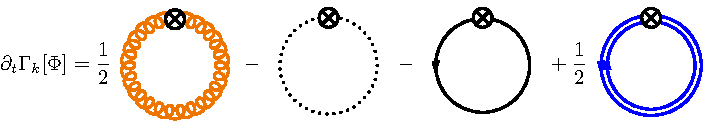
\includegraphics[width=0.45\textwidth]{QCD_equation}
\caption{Diagrammatic representation of the QCD flow equation within the fRG approach. Lines of different types on the r.h.s. of the equation stand for the full propagators of gluon, ghost, quark, and meson, respectively. Note that the mesonic degree of freedom is denoted by double lines with opposite arrows. The crossed circles represent the regulators in the flow equation.}\label{fig:QCD_equation}
\end{figure}
%%%%%%%%%%%%%%%%%%%%%%%%%%%%%
%

A generic quantum field theory is completely described by its effective action $\Gamma[\Phi]$, where $\Phi$ is used to denote the collection of all fields in the theory. In the fRG approach, this full quantum effective action is resolved by  
interpolating it as a function of a renormalization group (RG) scale $k$, i.e., $\Gamma_k[\Phi]$, successively, starting from the respective classical action $S[\Phi]$ at a very high ultraviolet (UV) scale, say $\Lambda$, towards the infrared (IR) limit $k\rightarrow 0$ with $\Gamma[\Phi]=\Gamma_{k=0}[\Phi]$. For more details about the formalism of fRG, see, e.g., \cite{Wetterich:1992yh} as well as \cite{Ellwanger:1993mw,Morris:1993qb}. 

To be specific, the flow equation for QCD, which describes the evolution of its effective action with the RG scale $k$, is shown in \Fig{fig:QCD_equation} diagrammatically. As one could see, the QCD flow receives contributions not only from the  gluon, ghost and the quark, i.e., the fundamental partonic degrees of freedom in QCD, but also from hadrons, such as mesons, which are composite or emergent degrees of freedom, and are generated dynamically through strong interactions when the RG scale is reduced down to the nonperturbative regime of the low energy QCD. Recent first-principle QCD calculations within fRG indicate that this transition, from the partonic to composite degrees of freedom, takes place in a narrow regime located at $k\sim$1 GeV \cite{Mitter:2014wpa,Braun:2014ata,Cyrol:2017ewj,Fu:2019hdw}. The flow of the QCD effective action corresponding to the diagrams in \Fig{fig:QCD_equation} can be written as follows,
%
\begin{align}
\partial_t\Gamma_k[\Phi]=&\frac{1}{2}\mathrm{Tr}\Big(G_{AA,k}\partial_t R_{A,k}\Big)-\mathrm{Tr}\Big(G_{c\bar c,k}\partial_t R_{c,k}\Big)\nonumber\\[2ex]
  &-\mathrm{Tr}\Big(G_{q\bar q,k}\partial_t R_{q,k}\Big)+\frac{1}{2}\mathrm{Tr}\Big(G_{\phi\phi,k}\partial_t R_{\phi,k}\Big)\,,\label{eq:QCDflow}
\end{align}
%
with $\Phi=(A, c, \bar c, q,\bar q,\phi)$, where $G$'s and $R$'s are the propagators and regulators of different fields, respectively. Note that the scale dependence of these quantities is explicitly indicated with a suffix $k$. The RG time in \Eq{eq:QCDflow} is defined by $t=\ln(k/\Lambda)$, with the initial UV scale $\Lambda$. We are not going to discuss details of the QCD flow in \Eq{eq:QCDflow} here, and interested readers are strongly suggested to refer to, e.g.,  \cite{Braun:2007bx,Braun:2008pi,Braun:2009gm,Mitter:2014wpa,Braun:2014ata,Cyrol:2016tym,Cyrol:2017ewj,Cyrol:2017qkl,Fu:2019hdw,Braun:2020ada} for recent progress in understanding of QCD or Yang-Mills theory in the vacuum and at finite temperature and density within the fRG approach, and also \cite{Berges:2000ew,Pawlowski:2005xe,Schaefer:2006sr,Gies:2006wv,Rosten:2010vm,Braun:2011pp,Pawlowski:2014aha,Dupuis:2020fhh} for QCD related review articles of fRG.

As mentioned above, the transition of the degrees of freedom, from the partonic ones in the perturbative regime of high energy to the hadronic ones in the nonperturbative region of low energy, is realized through the dynamical hadronization in the fRG approach. With the help of the technique of dynamical hadronization, composite operators of resonated channels, e.g., the $\sigma$-$\pi$ channel, i.e., the scalar-pseudoscalar one in the low energy QCD, which are most relevant to the dynamics of the system, are bosonized or Hubbard-Stratonovich transformed successively with the evolution of RG scale. For more details, see, e.g., \cite{Gies:2001nw,Gies:2002hq,Pawlowski:2005xe,Floerchinger:2009uf,Fu:2019hdw}. 

In a recent first-principle fRG calculation to QCD, it has been shown clearly that a sequential decoupling of the gluon, quark, and mesonic degrees of freedom from the system with decreasing RG scale, results in a natural emergence of the low energy effective theory (LEFT) when the scale $k\lesssim 1$ GeV \cite{Fu:2019hdw}. The fRG formalism is ideally suited to the description of a phenomenon of emergence, which usually involves energy scale of different hierarchies, characteristic to different degrees of freedom. When the scale $k$ is high and the system is located in the perturbative region, the only relevant degrees of freedom in QCD are the gluon and quark, and the hadronic or mesonic ones are irrelevant due to their large masses. When $k$ decreases below $\sim 1$ GeV, the gluon develops a significant mass gap in the low momentum region, and thus decouples from the system. The dynamics is taken over by the emergent composite degrees of freedom, e.g. mesons, in particular the $\pi$ meson, which is in essence the Goldstone boson related to the spontaneously breaking chiral symmetry in the low energy QCD, and is the lightest hadron of mass $\sim 140$ MeV in the vacuum. 

The direct consequence of the natural emergence of LEFT is that,  if the flow equation of QCD in \Eq{eq:QCDflow} is evolved from an initial scale where the glue sector has already been suppressed significantly by the gluon mass gap, \colfab{say $\Lambda < 1$ GeV}, it is safe and legitimate to disregard quantum fluctuations of the glue sector, i.e., the first two diagrams in \Fig{fig:QCD_equation}. Hence we are left with a scale dependent effective action in Euclidean spacetime, only composed of the dynamical matter fields, namely quarks and mesons, which reads
%
\begin{align}
\Gamma_k[\Phi]=&\int_x \bigg\{Z_{q,k}\bar{q} \Big [\gamma_\mu \partial_\mu -\gamma_0(\hat\mu+igA_0) \Big ]q+\frac{1}{2}Z_{\phi,k}(\partial_\mu \phi)^2 \nonumber\\[2ex]
&+h_k\bar{q}\big(T^0\sigma+i\gamma_5\vec{T}\cdot \vec{\pi}\big)q+V_k(\rho,A_0)-c\sigma \bigg\}\,,\label{eq:action}
\end{align}
%
with a reduction of the involved species of fields $\Phi=(q,\bar q,\phi)$, and the shorthand notation for the space-time integral $\int_{x}=\int_0^{1/T}d x_0 \int d^3 x$. Note that in this work we only consider the case of $N_f=2$ flavor quark, i.e., the quark field $q=(u\,,d)^{T}$ in the action \Eq{eq:action}. The meson field $\phi=\left(\sigma,\vec{\pi}\right)$, being in the adjoint representation of group $\mathrm{U_V}(N_f)\times\mathrm{U_A}(N_f)$ in the flavor space, is coupled with the quark field through the Yukawa coupling. Here $T^0$ and $T^{i}$'s ($i=1\,,2\,,\cdots\,,N_f^2-1$) are the generators of $\mathrm{U}(N_f)$ group, denoted collectively as $T^a$'s, with the normalization $\Tr(T^{a}T^{b})=\frac{1}{2}\delta^{ab}$, which yields $T^{0}=\frac{1}{\sqrt{2N_{f}}}\mathbb{1}_{N_{f}\times N_{f}}$. $Z_{q,k}$ and $Z_{\phi,k}$ are the wave function renormalization for the quark and meson fields, respectively. Note that the wave function renormalizations, as well as the Yukawa coupling $h_k$ and the effective potential $V_k$ to be discussed in the following, are dependent on the RG scale $k$. 

Quantum fluctuations of the glue sector are suppressed in the low energy region due to the large gluon mass gap as discussed above. Consequently, it is reasonable to neglect their corresponding contributions in the flow equation of QCD in \Fig{fig:QCD_equation} or \Eq{eq:QCDflow}, \colfab{provided that the initial scale is low enough and the initial effective action is chosen properly \cite{Rennecke:2015lur, Springer:2016cji, Alkofer:2018guy, Fu:2019hdw}}. The gluonic background field is, however, of significant importance for the thermodynamic properties of QCD. In \Eq{eq:action} the temporal component of the gluonic background field $A_0$ is encoded, which is responsible for the quark confinement in the statistical sense of thermodynamics, see, e.g., \cite{Fukushima:2003fw,Ratti:2005jh,Schaefer:2007pw,Fu:2007xc} for more details. Therefore, the effective potential in \Eq{eq:action} reads
%
\begin{align}
V_k(\rho,A_0)=&V_{\mathrm{glue},k}(A_0)+V_{\mathrm{mat},k}(\rho,A_0)\,,\label{eq:Vtotal}
\end{align}
%
where the first term on the right-hand side is due to the temporal gluonic background field $A_0$, which can also be formulated in terms of the Polyakov loop $L(A_0)$. More details about $V_{\mathrm{glue},k}$ used in this work can be found in \app{app:gluepot}. The matter part of the effective potential $V_{\mathrm{mat},k}$ arises from the quark and meson diagrams in \Fig{fig:QCD_equation}, which is dependent on the meson field through $\rho=\phi^2/2$. Clearly,   $V_{\mathrm{mat},k}$ is $\mathrm{SU_A}(2)$ or $\mathrm{O}(4)$ invariant, which guarantees that the chiral symmetry is preserved on the level of interactions. The explicit breaking of the chiral symmetry is attributed to the linear term $-c\sigma$ in \Eq{eq:action}, which is also related to a nonvanishing value of the current quark mass. The quark chemical potential $\hat\mu=\mathrm{diag}(\mu_u,\mu_d)$ in the first line of \Eq{eq:action} is a diagonal matrix in the flavor space, and $\mu=\mu_u=\mu_d$ is assumed throughout this work. The quark chemical potential is related to the baryon chemical potential via $\mu=\mu_B/3$.

In the scale regime of LEFT, as we have discussed above, the flow equation of the effective action in \Eq{eq:QCDflow} is reduced to 
%
\begin{align}
\partial_t\Gamma_k[\Phi]=&-\mathrm{Tr}\Big(G_{q\bar q,k}\partial_t R_{q,k}\Big)+\frac{1}{2}\mathrm{Tr}\Big(G_{\phi\phi,k}\partial_t R_{\phi,k}\Big)\,,\label{eq:LEFTflow}
\end{align}
%
where $R_{q,k}$ and $R_{\phi,k}$ are the regulators for the quark and meson fields, respectively. In this work we employ the $3d$- flat regulators \cite{Litim:2000ci, Litim:2001up, Litim:2006ag}, as follows
\begin{align}
  R_{\phi,k}(q_0,\bm{q})&=Z_{\phi,k}\bm{q}^2 r_B(\bm{q}^2/k^2)\,, \label{eq:Rphi}\\[2ex] 
  R_{q,k}(q_0,\bm{q})&=Z_{q,k}i\bm{\gamma} \cdot \bm{q} r_F(\bm{q}^2/k^2)\,, \label{eq:Rq}
\end{align} 
with 
\begin{align}
  r_B(x)&=\left( \frac{1}{x}-1 \right)\Theta(1-x)\,,\\[2ex] 
  r_F(x)&=\left( \frac{1}{\sqrt{x}}-1 \right)\Theta(1-x)\,,  \label{}
\end{align} 
where $\Theta(x)$ denotes the Heaviside step function. The full propagators read
%
\begin{align}
G_{q\bar q/\phi\phi,k}=&\left(\frac{1}{\Gamma^{(2)}_k[\Phi]+R_k}\right)_{q\bar q/\phi\phi}\,,\label{}
\end{align}
%
with $\Gamma^{(2)}_k[\Phi]=\delta^2\Gamma_k[\Phi]/(\delta \Phi_{i_1}\delta \Phi_{i_2})$, where different species of fields are distinguished with the help of the subscripts in $\Phi_{i_1/i_2}$. Inserting the effective action \eq{eq:action} into the flow equation \eq{eq:LEFTflow}, one is led to the flow equation for the effective potential of the matter sector, as follows
%
\begin{align}
  \partial_t V_{\mathrm{mat},k}(\rho)=&\frac{k^4}{4\pi^2} \bigg [\big(N^2_f-1\big) l^{(B,4)}_{0}(\tilde{m}^{2}_{\pi,k},\eta_{\phi,k};T)\nonumber\\[2ex]
&+l^{(B,4)}_{0}(\tilde{m}^{2}_{\sigma,k},\eta_{\phi,k};T)\nonumber\\[2ex]
&-4N_c N_f l^{(F,4)}_{0}(\tilde{m}^{2}_{q,k},\eta_{q,k};T,\mu)\bigg]\,, \label{eq:flowV}
\end{align}
%
where the threshold functions $l^{(B/F,4)}_{0}$ as well as other threshold functions in the following can be found in e.g., \cite{Fu:2019hdw,Yin:2019ebz}, and the dimensionless renormalized quark and meson masses read
%
\begin{align}
  \tilde{m}^{2}_{q,k}=&\frac{h^{2}_{k}\rho}{2k^2Z^{2}_{q,k}}\,, \qquad \tilde{m}^{2}_{\pi,k}=\frac{V'_{\mathrm{mat},k}(\rho)}{k^2 Z_{\phi,k}}\,, \\[2ex]
  \tilde{m}^{2}_{\sigma,k}=&\frac{V'_{\mathrm{mat},k}(\rho)+2\rho V''_{\mathrm{mat},k}(\rho)}{k^2 Z_{\phi,k}}\,.\label{}
\end{align}
%

The anomalous dimensions for the quark and meson fields in \Eq{eq:flowV} are defined as
%
\begin{align}
 \eta_{q,k}&=-\frac{\partial_t Z_{q,k}}{Z_{q,k}}\,,\qquad
  \eta_{\phi,k}=-\frac{\partial_t Z_{\phi,k}}{Z_{\phi,k}}\,,
\end{align}
%
respectively. Accordingly, projecting the flow in \Eq{eq:LEFTflow} onto the one-particle irreducible (1PI) two-point function of the meson, it is readily obtained that 
%
\begin{align}
  \eta_{\phi,k}&=-\frac{1}{3Z_{\phi,k}}\delta_{ij}\frac{\partial}{\partial (|\bm{p}|^2)}\frac{\delta^2 \partial_t \Gamma_k}{\delta \pi_i(-p) \delta \pi_j(p)}\Bigg|_{\substack{p_0=0\\ \bm{p}=0}}\,,\label{eq:etaphi}
\end{align}
%
where the spacial component is employed. Note that in the case of finite temperature and density, the $\mathrm{O}(4)$ rotation symmetry in the 4-$d$ Euclidean space is broken, and as a matter of fact, the mesonic anomalous dimension extracted above is different from that projected onto the temporal component. In another word, $\eta_{\phi,k}$ is split into $\eta_{\phi,k}^{\perp}$ and $\eta_{\phi,k}^{\parallel}$, which are transverse and longitudinal to the heat bath, respectively, at finite temperature and density. The influences of the splitting of $\eta_{\phi,k}$ on the thermodynamics and baryon number fluctuations have been investigated in detail \cite{Yin:2019ebz}, and it has been found that the impact is small. Therefore, it is reasonable to disregard the splitting of anomalous dimensions, and $\eta_{\phi,k}=\eta_{\phi,k}^{\perp}=\eta_{\phi,k}^{\parallel}$, as well as that for the quark anomalous dimension in the following, is assumed throughout this work. In the same way, the quark anomalous dimension is obtained by projecting the relevant flow onto the vector channel of the 1PI quark-antiquark correlation function, as follows
%
\begin{align}
  \eta_{q}&=\frac{1}{4 Z_{q,k}}\nonumber\\[2ex]
&\times\mathrm{Re}\left[\frac{\partial}{\partial (|\bm{p}|^2)}\mathrm{tr}
            \left(i \bm{\gamma}\cdot\bm{p}\left(-\frac{\delta^2}{\delta\bar{q}(p)
            \delta q(p)}\partial_t \Gamma_k\right)\right)\right]\Bigg|_{\substack{p_{0,ex}\\ \bm{p}=0}}\,,  \label{eq:etapsi}
\end{align}
%
where the external spacial momentum is chosen to be zero as same as the mesonic one, since the vanishing momentum is most relevant to the flow of effective potential in \Eq{eq:flowV}. Note that the lowest mode of the fermionic Matsubara frequency is nonvanishing and we designate it here as $p_{0,ex}$, to be described in \app{app:flowV}. Moreover, the expression in the square bracket in \eq{eq:etapsi} is complex-valued, rather than real, when the chemical potential is nonzero. This artifact stems from the naive truncation of the external frequency, which is resolved through a resummation of the external frequency of the quark propagator \cite{Fu:2016tey}. The flow equation of the Yukawa coupling is readily obtained via the projection of the 1PI quark-antiquark correlation function on the scalar channel, which reads
%
\begin{align}
  \partial_t h_k&=\frac{1}{2 \sigma}\mathrm{Re}\left[\mathrm{tr}\left(-\frac{\delta^2}{\delta\bar{q}(p)
            \delta q(p)}\partial_t \Gamma_k\right)\right]\Bigg|_{\substack{p_{0,ex}\\ \bm{p}=0}}\,.  \label{eq:dth}
\end{align}
%
The explicit expressions for the meson and quark anomalous dimensions, and the flow of the Yukawa coupling can be found in \app{app:flowV}.

%%%%%%%%%%%%%%%%%%%%%%%%%%%%%%%%%%%%%%%%%%%%%%%%%%%%%%%%%%%%%
%%%%%%%%%%%%%%%%%%%%%%%%%%%%%%%%%%%%%%%%%%%%%%%%%%%%%%%%%%%%%

\section{Thermodynamics and Hyper-order baryon number fluctuations}
\label{sec:hyper-fluc}

The thermodynamical potential density in the LEFT at finite temperature and nonzero baryon chemical potential is readily obtained from the effective action in \Eq{eq:action}, which reads
%
\colfab{
\begin{align}
  \Omega[T,\mu_B]=&V_{\mathrm{glue}}(L, \bar L)+V_{\mathrm{mat},k=0}(\rho, L, \bar L)-c\sigma\,,\label{eq:Omega}
\end{align}
}
%
where the gluonic background field $A_0$ has been reformulated in terms of the Polyakov loop $L$ and its complex conjugate $\bar L$. The matter sector of the effective potential is integrated out towards the IR limit $k=0$, while the glue sector is independent of $k$, see \app{app:gluepot}. Note that the Polyakov loop and the meson field are on their respective equations of motion, and the effective potential in \Eq{eq:Omega} is normalized to zero in vacuum. The pressure of the system is directly related to the thermodynamical potential, as follows
%
\begin{align}
  p=&-\Omega[T,\mu_B]\,.\label{eq:pres}
\end{align}
%
The generalized susceptibility of the baryon number $\chi^B_n$ is defined through the $n$-order derivative of the pressure w.r.t. the baryon chemical potential, to wit,
%
\begin{align}
  \chi_n^{B}&=\frac{\partial^n}{\partial (\mu_B/T)^n}\frac{p}{T^4}\,.\label{eq:suscept}
\end{align}
%
The generalized susceptibilities are related to various cumulants of the baryon number distribution, which can be measured in heavy-ion collision experiments through the cumulants of its proxy, i.e., the net proton distribution, see, e.g. \cite{Luo:2017faz} for details. For the lowest four orders, one is led to
%
\begin{align}
\chi^B_1=&\frac{1}{VT^3}\braket{N_B}\,,\quad \chi^B_2=\frac{1}{VT^3}\braket{(\delta N_B)^2}\,,\label{eq:chiB1}\\[2ex]
\chi^B_3=&\frac{1}{VT^3}\braket{(\delta N_B)^3}\,,\\[2ex]
\chi^B_4=&\frac{1}{VT^3}\Big(\braket{(\delta N_B)^4}-3\braket{(\delta N_B)^2}^2\Big)\,,\label{eq:chiB4}
\end{align}
%
with $\braket{\cdots}$ denoting the ensemble average and $\delta N_B=N_B-\braket{N_B}$. Thus the mean value of the net baryon number of the system is given by $M=VT^3\chi_1^{B}$, the variance $\sigma^2=VT^3\chi_2^{B}$, skewness $S=\chi_3^{B}/(\chi_2^{B}\sigma)$, and the kurtosis $\kappa=\chi_4^{B}/(\chi_2^{B}\sigma^2)$, respectively.

In this work emphasis is, however, put on the baryon number fluctuations of order higher than the fourth, i.e., $\chi_n^{B}$'s ($n>4$), which are named hyper-order baryon number fluctuations. As same as the low-order ones, the hyper-order susceptibilities are also connected to their respective cumulants, and their relations, taking the fifth through eighth ones for instance, are given as follows
%
\begin{align}
\chi^B_5=&\frac{1}{VT^3}\Big(\braket{(\delta N_B)^5}-10\braket{(\delta N_B)^2}\braket{(\delta N_B)^3}\Big)\,,\\[2ex]
\chi^B_6=&\frac{1}{VT^3}\Big(\braket{(\delta N_B)^6}-15\braket{(\delta N_B)^4}\braket{(\delta N_B)^2}\nonumber\\[2ex]
&-10\braket{(\delta N_B)^3}^2+30\braket{(\delta N_B)^2}^3\Big)\,,
\end{align}
\begin{align}
\chi^B_7=&\frac{1}{VT^3}\Big(\braket{(\delta N_B)^7}-21\braket{(\delta N_B)^5}\braket{(\delta N_B)^2}\nonumber\\[2ex]
&-35\braket{(\delta N_B)^4}\braket{(\delta N_B)^3}\nonumber\\[2ex]
&+210\braket{(\delta N_B)^3}\braket{(\delta N_B)^2}^2\Big)\,,\\[2ex]
\chi^B_8=&\frac{1}{VT^3}\Big(\braket{(\delta N_B)^8}-28\braket{(\delta N_B)^6}\braket{(\delta N_B)^2}\nonumber\\[2ex]
&-56\braket{(\delta N_B)^5}\braket{(\delta N_B)^3}-35\braket{(\delta N_B)^4}^2\nonumber\\[2ex]
&+420\braket{(\delta N_B)^4}\braket{(\delta N_B)^2}^2\nonumber\\[2ex]
&+560\braket{(\delta N_B)^3}^2\braket{(\delta N_B)^2}-630\braket{(\delta N_B)^2}^4\Big)\,.
\end{align}
%
\colfab{Different aspects of hyper-order fluctuations have been studied in mean-field approximations in the past, see e.g.\ \cite{Wagner:2009pm, Karsch:2010hm, Schaefer:2011ex}. However, due to the decisive role that non-perturbative quantum fluctuations play for these quantities, a treatment beyond mean-field, as in the present work, is necessary for their accurate description.}


%%%%%%%%%%%%%%%%%%%%%%%%%%%%%%%%%%%%%%%%%%%%%%%%%%%%%%%%%%%%%
%%%%%%%%%%%%%%%%%%%%%%%%%%%%%%%%%%%%%%%%%%%%%%%%%%%%%%%%%%%%%

\section{Numerical results and discussions}
\label{sec:num}

%
%%%%%%%%%%%%%%%%%%%%%%%%%%%%%
\begin{figure*}[t]
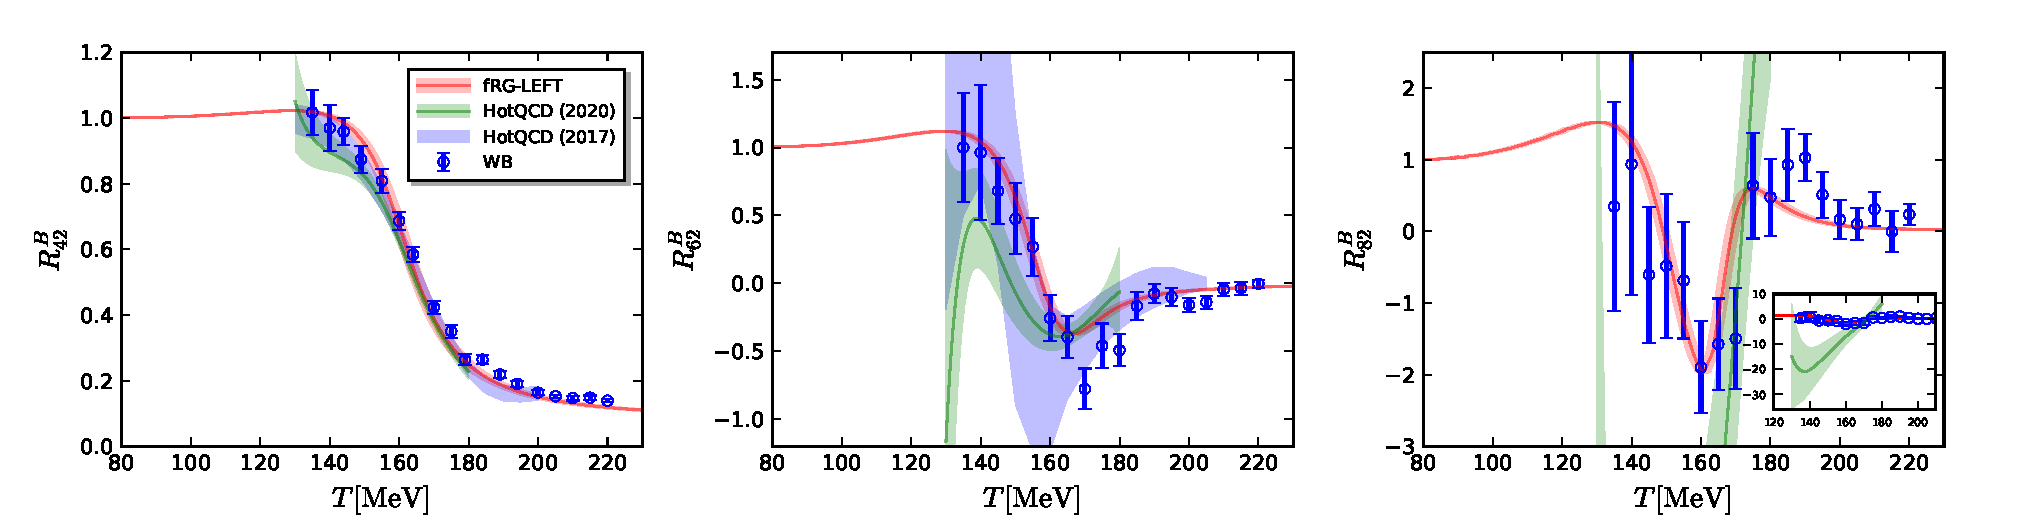
\includegraphics[width=1\textwidth]{R42R62R82-T-muB0}
\caption{$R^{B}_{42}=\chi^{B}_{4}/\chi^{B}_{2}$ (left panel), $R^{B}_{62}=\chi^{B}_{6}/\chi^{B}_{2}$ (middle panel), and $R^{B}_{82}=\chi^{B}_{8}/\chi^{B}_{2}$ (right panel) as functions of the temperature with vanishing baryon chemical potential ($\mu_B=0$). Results obtained with the low energy effective theory within fRG approach are compared with lattice results from the HotQCD collaboration \cite{Bazavov:2017dus,Bazavov:2017tot,Bazavov:2020bjn} and the Wuppertal-Budapest collaboration \cite{Borsanyi:2018grb}. The inset in the plot of $R^{B}_{82}$ shows its zoom-out view.}\label{fig:R42R62R82-T-muB0}
\end{figure*}
%%%%%%%%%%%%%%%%%%%%%%%%%%%%%
%

%
 %%%%%%%%%%%%%%%%%%%%%%%%%%%%
\begin{figure}[t]
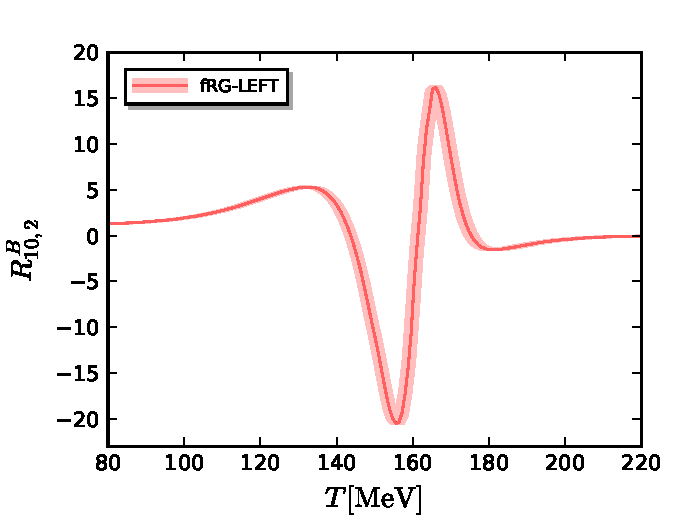
\includegraphics[width=0.45\textwidth]{R102-T-muB0}
\caption{$R^{B}_{10,2}=\chi^{B}_{10}/\chi^{B}_{2}$ as a function of the temperature with $\mu_B=0$, predicted by the LEFT within the fRG approach.}\label{fig:R102-T-muB0}
\end{figure}
%%%%%%%%%%%%%%%%%%%%%%%%%%%%%
%



In this section we would like to present our calculated results and compare them with the relevant lattice calculations. Implications of our prediction for the hyper-order baryon number fluctuations in the heavy-ion collision experiments will also be discussed. But before we do that, the scales in the LEFT and OCD have to be matched.

\subsection{Matching the scales in LEFT and OCD}
\label{subsec:scale}

Usually the scale in LEFT and that in QCD do not agree with each other exactly, and a direct consequence is that the pseudocritical temperature of the chiral phase crossover, i.e., the value of $T_c$ at $\mu_B=0$ is different in the LEFT and QCD. Although it is not a real phase transition, the benchmark value of $T_c$ is well determined through, e.g., the chiral condensate, chiral susceptibilities, etc. Recently, two lattice collaborations, the HotQCD collaboration and the Wuppertal-Budapest collaboration find $T_c=156.5\pm 1.5$ MeV \cite{Bazavov:2018mes} and $T_c=158.0\pm 0.6$ MeV, respectively. Furthermore, the scale is also affected by the number of quark flavors. As shown in the effective action in \Eq{eq:action}, only the $N_f=2$ flavor quarks, i.e., light quarks $u$ and $d$, are included in the LEFT in this work, while in lattice simulations besides the light quarks, dynamics of the strange quark is also taken into account. Thus there should be a mismatch of the scale resulting from the different systems of $N_f=2$ and $N_f=2+1$ flavor quarks.

We denote the temperature and the baryon chemical potential in the LEFT as $T_{_{LEFT}}$ and $\mu_{B_{LEFT}}$, respectively, where the suffix is used to distinguish them from $T$ and $\mu_{B}$ in QCD or lattice simulations. In order to resolve the mismatch of the scale in LEFT and OCD, a simple linear relation between them both for the temperature and chemical potential is assumed, to wit,
%
\begin{align}
  T_{_{LEFT}}&=c_{_{T}}T\,, \quad \mu_{B_{LEFT}}=c_{\mu}\mu_{B}\,,\label{eq:rescale}
\end{align}
%
where the constant coefficients $c_{_{T}}$ and $c_{\mu}$ are to be determined.

The coefficient $c_{_{T}}$ in \Eq{eq:rescale} is fixed through fitting the LEFT curve of $R^{B}_{42}=\chi^{B}_{4}/\chi^{B}_{2}$ in the left panel of \Fig{fig:R42R62R82-T-muB0}, i.e., the kurtosis of the baryon number distribution $\kappa \sigma^2=R^{B}_{42}$, 
as a function of the physical temperature $T$ with $\mu_B=0$ in comparison to the lattice results. It is found that the LEFT within fRG provides the best description of the lattice $\kappa \sigma^2$ with $c_{_{T}}=1.247(12)$. To proceed, the constant $c_{\mu}$ in \Eq{eq:rescale} is determined by the curvature of the phase boundary, which is defined as the quadratic expansion coefficient of the pseudocritical temperature as a function of the baryon chemical potential around $\mu_B=0$, i.e.,
%
\begin{align}
  \frac{T_c(\mu_B)}{T_c}&=1-\kappa \left(\frac{\mu_B}{T_c}\right)^2+\lambda \left(\frac{\mu_B}{T_c}\right)^4+\cdots\,,\label{eq:curv}
\end{align}
%
with the curvature $\kappa$, where the next fourth order expansion coefficient $\lambda$ is neglected in our calculations, since it hardly plays any role in the region of baryon chemical potential concerned in this work, e.g., up to $\mu_B\sim 400$ MeV in the following, due to its small value. $T_c$ in \Eq{eq:curv} is the pseudocritical temperature at $\mu_B=0$. Note that the curvature is invariant only if the chemical potential and temperature are rescaled with the same value, and thus the curvature $\kappa_{_{LEFT}}$ in the LEFT would not be modified if one has $c_{\mu}=c_{_{T}}$ in \Eq{eq:rescale}. By employing the order parameter of the chiral phase transition, i.e., the expectation value of the sigma field $\langle \sigma \rangle$ in \Eq{eq:action}, we obtain $\kappa_{_{LEFT}}=0.0193$ in the $N_f=2$ flavor LEFT. For more discussions about the phase boundary and curvature, see, e.g., \cite{Fu:2019hdw}. This value of $\kappa_{_{LEFT}}$ is a bit larger than recent $N_f = 2+1$ lattice results, e.g., $\kappa=0.015(4)$ in \cite{Bazavov:2018mes}, $\kappa=0.0149(21)$ in \cite{Bellwied:2015rza}, $\kappa=0.0153(18)$ in \cite{Borsanyi:2020fev}. This mismatch of the curvature between the LEFT and lattice QCD, however, is cured through a suitable choice for the ratio $c_{\mu}/c_{_{T}}$ in \Eq{eq:rescale}, and one readily arrives at
%
\begin{align}
  c_{\mu}&=c_{_{T}}\left(\frac{\kappa}{\kappa_{_{LEFT}}}\right)^{1/2}\,.\label{eq:cmu}
\end{align}
%
Substituting $\kappa_{_{LEFT}}=0.0193$, $\kappa=0.0153(18)$, and $c_{_{T}}=1.247(12)$ into the equation above, one obtains $c_{\mu}=1.110(66)$.
\colfab{The errors on our results in the following reflect the uncertainties on these parameters. [Is this correct or did I miss something?]}

To sum up, in this section the scales between the LEFT and QCD have been matched by resorting to two observables, i.e., $R^{B}_{42}$ as a function of $T$ at vanishing chemical potential and the curvature of phase boundary $\kappa$, which are both quite relevant to predictions of the hyper-order baryon number fluctuations at finite temperature and densities, to be discussed in the following. 


%%%%%%%%%%%%%%%%%%%%%%%%%%%%%%%%%%%%%%%%%%%%%%%%%%%%%%%%%%%%%
\subsection{Hyper-order baryon number fluctuations}
\label{subsec:hyper-order}

%
%%%%%%%%%%%%%%%%%%%%%%%%%%%%%
%\begin{figure*}[t]
%\centering
%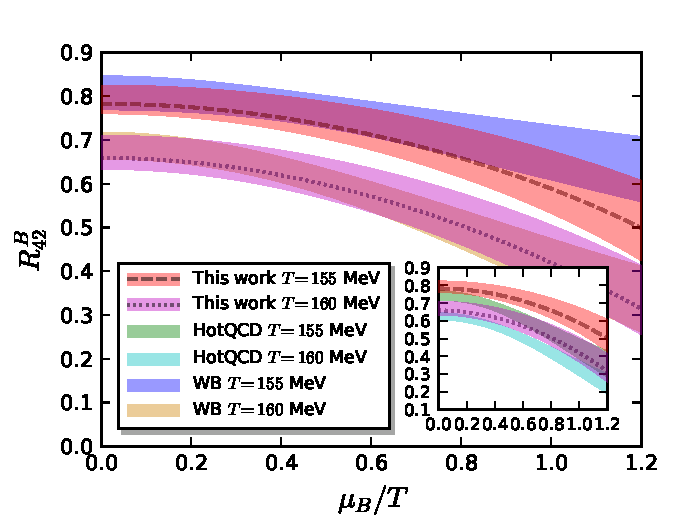
\includegraphics[width=0.85\columnwidth]{R42-muBoT} 
%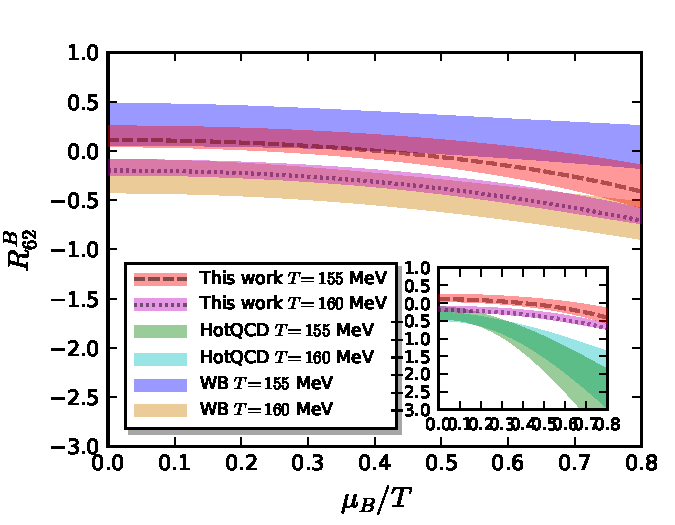
\includegraphics[width=0.85\columnwidth]{R62-muBoT} 
%\caption{$R^{B}_{42}$ (left panel) and $R^{B}_{62}$ (right panel) as functions of $\mu_B/T$ with $T=155$ MeV and $T=160$ MeV. Calculation of LEFT within the fRG approach is compared with lattice QCD computations by the HotQCD collaboration \cite{Bazavov:2020bjn} and the Wuppertal-Budapest collaboration \cite{Borsanyi:2018grb}.
%} \label{fig:R42R62-muBoT}
%\end{figure*}
%%%%%%%%%%%%%%%%%%%%%%%%%%%%%
%

%
%%%%%%%%%%%%%%%%%%%%%%%%%%%%%
\begin{figure*}[t]
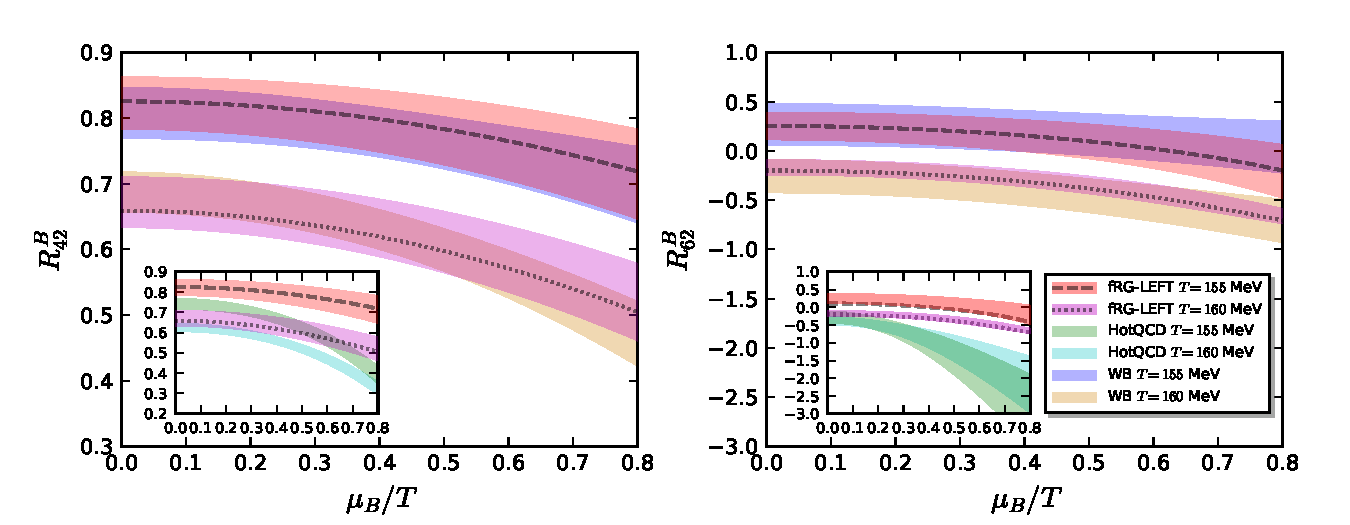
\includegraphics[width=0.9\textwidth]{R42R62-muBoT}
\caption{$R^{B}_{42}$ (left panel) and $R^{B}_{62}$ (right panel) as functions of $\mu_B/T$ with $T=155$ MeV and $T=160$ MeV. Calculation of LEFT within the fRG approach is compared with lattice QCD by the HotQCD collaboration \cite{Bazavov:2020bjn} and the Wuppertal-Budapest collaboration \cite{Borsanyi:2018grb}. Note that the comparison of $R^{B}_{42}$ between HotQCD and LEFT is presented in the inlays, in order to improve the readability of presentation.}\label{fig:R42R62-muBoT}
\end{figure*}
%%%%%%%%%%%%%%%%%%%%%%%%%%%%%
%

%
%%%%%%%%%%%%%%%%%%%%%%%%%%%%%
\begin{figure*}[t]
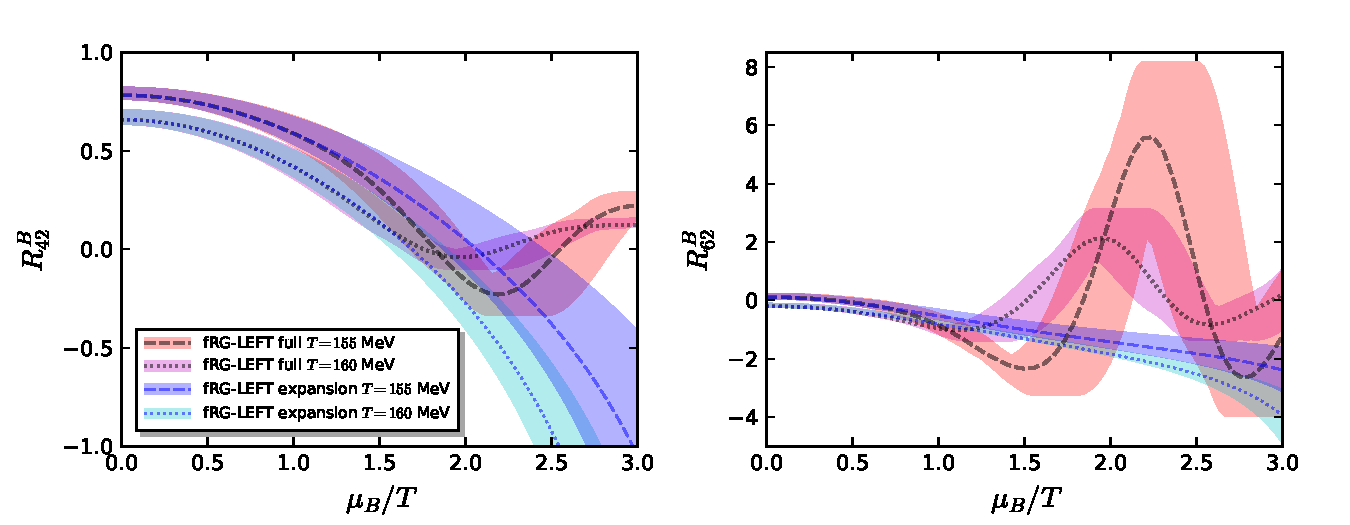
\includegraphics[width=0.9\textwidth]{R42R62expansion-muBoT}
\caption{Comparison between the direct full calculation of baryon number fluctuations $R^{B}_{42}$ (left panel) and $R^{B}_{62}$ (right panel) via \Eq{eq:suscept} and the Taylor expansion in Eqs. (\ref{eq:chiB2Tay})  (\ref{eq:chiB4Tay})  (\ref{eq:chiB6Tay}). Both calculations are performed within the LEFT-fRG approach, and $R^{B}_{42}$, $R^{B}_{62}$ are plotted as functions of $\mu_B/T$ with $T=155$ MeV and $T=160$ MeV.}\label{fig:R42R62expansion-muBoT}
\end{figure*}
%%%%%%%%%%%%%%%%%%%%%%%%%%%%%
%

%
%%%%%%%%%%%%%%%%%%%%%%%%%%%%%
\begin{figure*}[t]
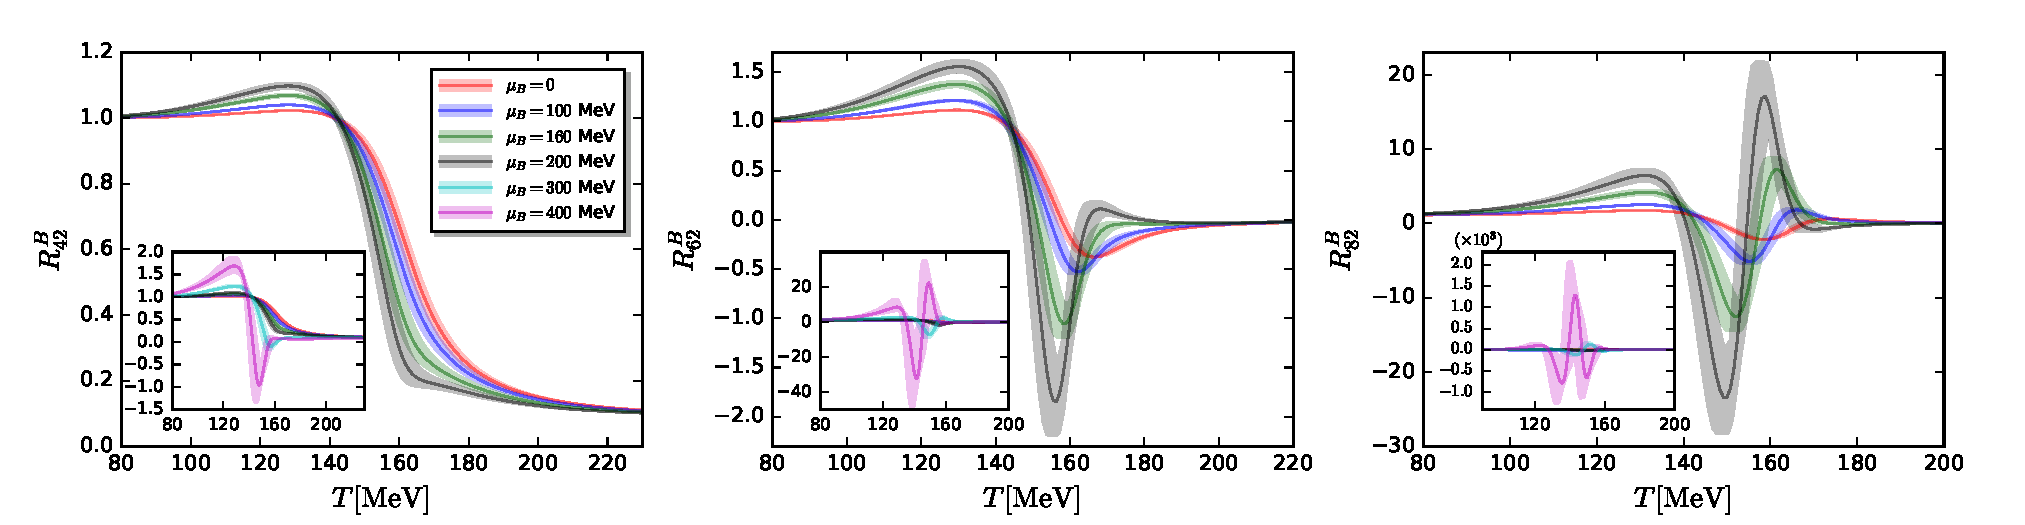
\includegraphics[width=1.\textwidth]{R42R62R82-T-muB0to400}
\caption{$R^{B}_{42}$ (left panel), $R^{B}_{62}$ (middle panel), and $R^{B}_{82}$ (right panel) as functions of the temperature at several values of $\mu_B$, computed from LEFT within the fRG approach. Insets in each plot show their respective zoom-out view.}\label{fig:R42R62R82-T-muB0to400}
\end{figure*}
%%%%%%%%%%%%%%%%%%%%%%%%%%%%%
%

As we have discussed above, the LEFT has been calibrated by use of the curvature of phase boundary and the kurtosis of baryon number distribution as a function of $T$ with $\mu_B=0$, via a detailed comparison with recent lattice results. Consequently, one could use the LEFT to make predictions for the dependence of $R^{B}_{42}$ on the chemical potential, as well as the hyper-order baryon number fluctuations at finite temperature and density. In the middle and right panels of \Fig{fig:R42R62R82-T-muB0}, $R^{B}_{62}=\chi^{B}_{6}/\chi^{B}_{2}$ and $R^{B}_{82}=\chi^{B}_{8}/\chi^{B}_{2}$ are shown versus the temperature with vanishing $\mu_B$, respectively, and in the same way the LEFT and lattice QCD results are compared. Apparently, one observes that, with the increase of the order of fluctuations, errors of lattice calculation increase dramatically. Specifically, the eighth-order fluctuations $R^{B}_{82}$ obtained by the two collaborations show a significant quantitative difference, although they are roughly consistent with each other qualitatively. It is found that the predicted hyper-order baryon number fluctuations from the LEFT within the fRG, are in qualitative agreement with both lattice results, and even consistent with the Wuppertal-Budapest result quantitatively within the errors.
\colfab{We also computed the hyper-order fluctuations within a simple hadron resonance gas model \cite{BraunMunzinger:2003zd} and found them to be essentially equal to one with only a very minor monotonic increase with $T$ for $T \lesssim 140$~MeV. This is in agreement with our findings.}
Moreover, we have also computed baryon number fluctuations of orders even up to the tenth in the LEFT, and the relevant result $R^{B}_{10,2}=\chi^{B}_{10}/\chi^{B}_{2}$ is presented in \Fig{fig:R102-T-muB0}, where the chemical potential is chosen to be vanishing. Note that no lattice results for the tenth-order fluctuation are available for the moment, and the dependence of $R^{B}_{10,2}$ on the temperature in \Fig{fig:R102-T-muB0} is a pure prediction by the LEFT within the fRG approach, which needs to be confirmed by other calculations, e.g., lattice QCD, in the future.

To proceed, we consider the chemical potential dependence of baryon number fluctuations. Expanding the pressure in \Eq{eq:pres} in powers of $\hat{\mu}_{B}\equiv\mu_B/T$ around $\hat{\mu}_{B}=0$ , one is led to 
%
\begin{align}
  \frac{p}{T^4}&=\frac{p}{T^4}\Big|_{\hat{\mu}_{B}=0}+\sum_{i=1}^{\infty}\frac{\chi^B_{2i}|_{\hat{\mu}_{B}=0}}{(2i)!}\hat{\mu}_{B}^{2i}\,.\label{eq:cmu}
\end{align}
%
Truncating the Taylor expansion above up to order of $\hat{\mu}_{B}^{8}$ and employing \Eq{eq:suscept}, we obtain the expanded baryon number fluctuations in the first several orders, to wit,
%
\begin{align}
\chi^B_2\simeq&\chi^B_2|_{\hat{\mu}_{B}=0}+\frac{\chi^B_4|_{\hat{\mu}_{B}=0}}{2!}\hat{\mu}_{B}^{2}+\frac{\chi^B_6|_{\hat{\mu}_{B}=0}}{4!}\hat{\mu}_{B}^{4}\nonumber\\[2ex]
&+\frac{\chi^B_8|_{\hat{\mu}_{B}=0}}{6!}\hat{\mu}_{B}^{6}\,,\label{eq:chiB2Tay}\\[2ex]
\chi^B_4\simeq&\chi^B_4|_{\hat{\mu}_{B}=0}+\frac{\chi^B_6|_{\hat{\mu}_{B}=0}}{2!}\hat{\mu}_{B}^{2}+\frac{\chi^B_8|_{\hat{\mu}_{B}=0}}{4!}\hat{\mu}_{B}^{4}\,,\label{eq:chiB4Tay}\\[2ex]
\chi^B_6\simeq&\chi^B_6|_{\hat{\mu}_{B}=0}+\frac{\chi^B_8|_{\hat{\mu}_{B}=0}}{2!}\hat{\mu}_{B}^{2}\,.\label{eq:chiB6Tay}
\end{align}
%
In \Fig{fig:R42R62-muBoT} we show the lattice results $\chi^B_4/\chi^B_2$ and $\chi^B_6/\chi^B_2$ based on the Taylor expansion above, and the fluctuations at vanishing chemical potential, viz. $\chi^B_{i}|_{\hat{\mu}_{B}=0}$ ($i=2$, 4, 6, 8) and relevant results in \Fig{fig:R42R62R82-T-muB0}, from the HotQCD collaboration \cite{Bazavov:2020bjn} and the Wuppertal-Budapest collaboration \cite{Borsanyi:2018grb}. Moreover, $\chi^B_n$'s in \Eq{eq:suscept} could also be computed directly in the LEFT within the fRG approach, without resorting to the Taylor expansion, and the relevant results are presented in \Fig{fig:R42R62-muBoT} for comparison. Here we choose two values of the temperature, and as expected, the LEFT result for the dependence of $R^{B}_{42}$ and $R^{B}_{62}$ on the chemical potential, agrees with both lattice results qualitatively, and is even quantitatively consistent with the Wuppertal-Budapest result. Moreover, it is of high interest to investigate the convergence of Taylor expansion in Eqs. (\ref{eq:chiB2Tay}) (\ref{eq:chiB4Tay}) (\ref{eq:chiB6Tay}), via a comparison to the full calculation of baryon number fluctuations in \Eq{eq:suscept}. We have done both calculations in the LEFT-fRG approach, and the relevant results are shown in \Fig{fig:R42R62expansion-muBoT}. One observes that the Taylor expansion in Eqs. (\ref{eq:chiB2Tay})  (\ref{eq:chiB4Tay})  (\ref{eq:chiB6Tay}), where it is expanded up to $\chi^B_8$ at vanishing baryon chemical potential for the $\mu_B$-dependence of baryon number fluctuations of lower orders, agrees with the full calculation for $R^{B}_{42}$ with $\mu_B/T$ going up to 1.2, but the convergence upper bound for the higher-order fluctuation $R^{B}_{62}$ is decreased to $\sim$ 0.8. We find that the full calculation of $R^{B}_{62}$ with $\mu_B/T \gtrsim 1.0$ deviates from that of Taylor expansion significantly.

In \Fig{fig:R42R62R82-T-muB0to400} $R^{B}_{42}$, $R^{B}_{62}$ and $R^{B}_{82}$ are depicted as functions of $T$ with several values of $\mu_B$, which are calculated in LEFT with the fRG approach. Relevant results in \Fig{fig:R42R62R82-T-muB0} for $\mu_B=0$ are presented as well, in order to highlight effects of the finite baryon chemical potential, whose value is increased from zero to 400 MeV. One observes that both the magnitude and error of the fluctuations, in particular the high-order ones, grow with the increasing chemical potential. Due to the rapid increase of error for very high-order fluctuations at large baryon chemical potential, e.g., $R^{B}_{82}$ with $\mu_B\gtrsim 200$ MeV, it is reasonable to expect that the LEFT is losing its capability of making predictions in these regimes.

%\begin{table}[t]
%  \begin{center}
%    \begin{tabular}{|c ||c|c|c|c|c|c|c|c|c|}
%    \hline & & & & & & & & & \\[-2ex]
%    \hline & & & & & & & & & \\[-1ex]
%    $\sqrt{s_{NN}}$ [GeV] & 200 & 62.4 & 54.4 & 39 & 27 & 19.6 & 14.5 & 11.5 & 7.7\\[1ex]
%    \hline & & & & & & & & & \\[-2ex]
%    ${\mu_B}_{_{CF}}$ [MeV] & 22 & 68 & 78 & 106 & 148 & 196 & 252 & 303 & 406\\[1ex]
%    \hline & & & & & & & & & \\[-2ex]
%    $T_{_{CF}}$ (I) [MeV] &158 & 158 & 158 & 158 & 157 & 156 & 153 & 150 & 138\\[1ex]
%    \hline & & & & & & & & & \\[-2ex]
%    $T_{c}$ [MeV] & 164 & 164 & 164 & 163 & 162 & 161 & 158 & 155 & 146\\[1ex]
%    \hline & & & & & & & & & \\[-2ex]
%    $T_{_{CF}}$ (II) [MeV] & 162 & 163 & 163 & 161 & 159 & 156 & 151 & 145 & 134\\[1ex]
%    \hline
%    \end{tabular}
%    \caption{Chemical freeze-out parameters ${\mu_B}_{_{CF}}$ and $T_{_{CF}}$ (freeze-out: I, II) for different center-of-mass energies per nucleon pair $\sqrt{s_{\mathrm{NN}}}$. See text for details.}
%    \label{tab:freeze-out-para}  
%  \end{center}\vspace{-0.5cm}
%\end{table}

%
%%%%%%%%%%%%%%%%%%%%%%%%%%%%%
\begin{figure}[t]
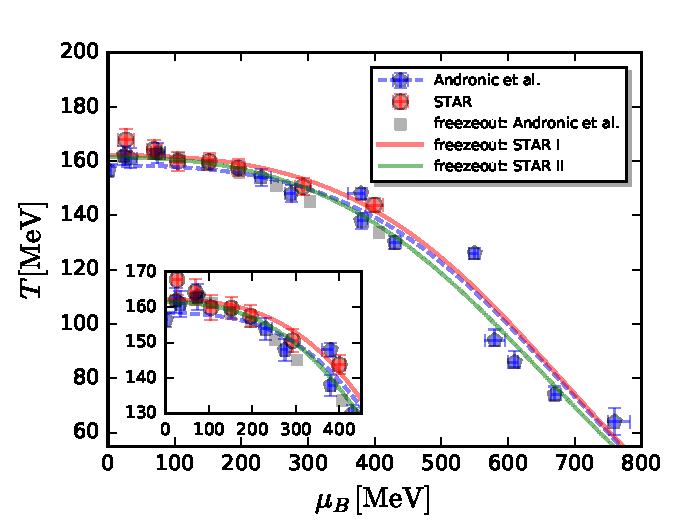
\includegraphics[width=0.48\textwidth]{phasediagram}
\caption{Chemical freeze-out temperature and baryon chemical potential in the $T-\mu_B$ plane. The blue pentagons and red circles show the freeze-out data from Andronic {\it et al.} \cite{Andronic:2017pug} and STAR experiment \cite{Adamczyk:2017iwn}, respectively. The blue dashed line represents the parametrization of blue pentagons through Eqs. (\ref{eq:muBCFparatri}) and (\ref{eq:TCFparatri}). The red solid and green dotted lines show the parametrization of the STAR data based on all the seven data points, and only the four data points in the middle region ($100\,\mathrm{MeV}\lesssim\mu_B\lesssim 300\,\mathrm{MeV}$), respectively. The gray squares are obtained by interpolating the blue pentagons. The inlay zooms in the low-$\mu_B$ region.}\label{fig:phasediagram}
\end{figure}
%%%%%%%%%%%%%%%%%%%%%%%%%%%%%
%

%
%%%%%%%%%%%%%%%%%%%%%%%%%%%%%
\begin{figure}[t]
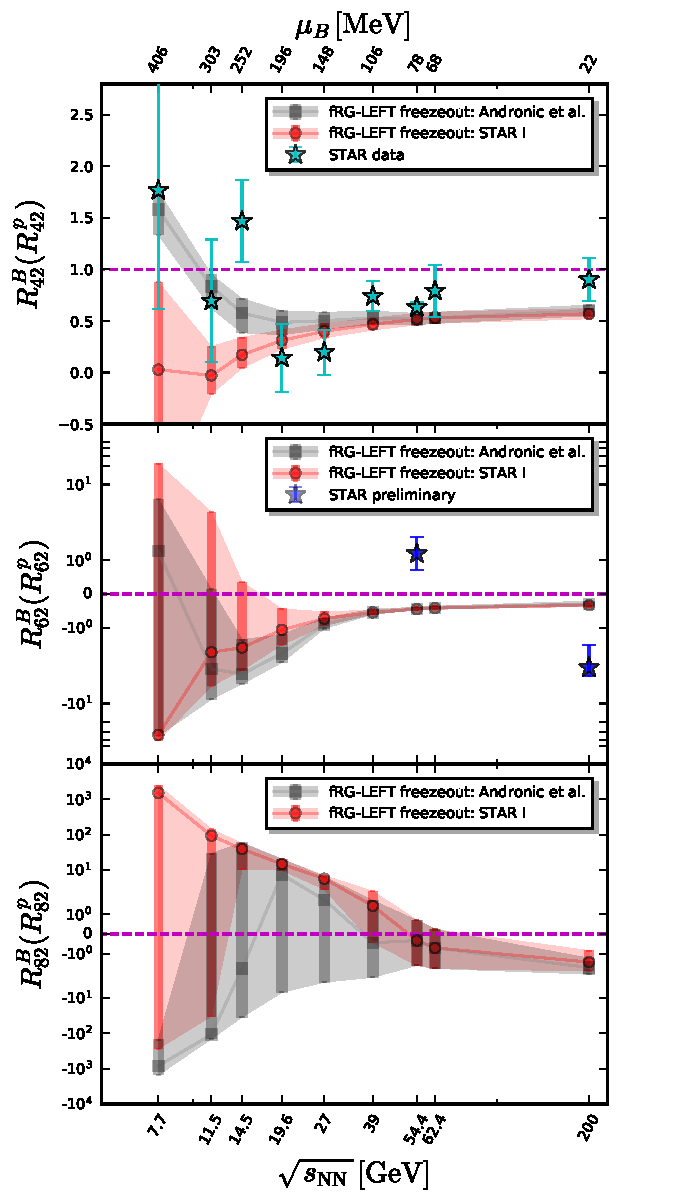
\includegraphics[width=0.45\textwidth]{Rm2-sqrtS}
\caption{Baryon number fluctuations $R^{B}_{42}$ (top), $R^{B}_{62}$ (middle), and $R^{B}_{82}$ (bottom) as functions of the collision energy, calculated in LEFT within the fRG approach with the freeze-out parameters from Andronic {\it et al.} \cite{Andronic:2017pug} and STAR experiment \cite{Adamczyk:2017iwn}, where the parametrization of STAR freeze-out data is based on all the seven data points as shown in \Fig{fig:phasediagram} and is designated as freezeout: STAR I. Experimental data of cumulants from the STAR collaboration are also shown for comparison, where $R^{p}_{42}$ (top) are the kurtosis of the net-proton distributions measured in Au+Au central (0-5\%) collisions \cite{Adam:2020unf}, and $R^{p}_{62}$ (middle) is the preliminary result on the six-order cumulant of the net-proton distribution at $\sqrt{s_{\mathrm{NN}}}$=200 GeV and 54.4 GeV with centrality 0-40\% \cite{Nonaka:2020crv,Pandav:2020uzx}. The horizontal dashed lines indicate positions of unity for $R^{B}_{42}$($R^{p}_{42}$), zeros for $R^{B}_{62}$($R^{p}_{62}$) and $R^{B}_{82}$.}\label{fig:Rm2-sqrtS}\vspace{-0.5cm}
\end{figure}
%%%%%%%%%%%%%%%%%%%%%%%%%%%%%
%

%
%%%%%%%%%%%%%%%%%%%%%%%%%%%%%
\begin{figure}[t]
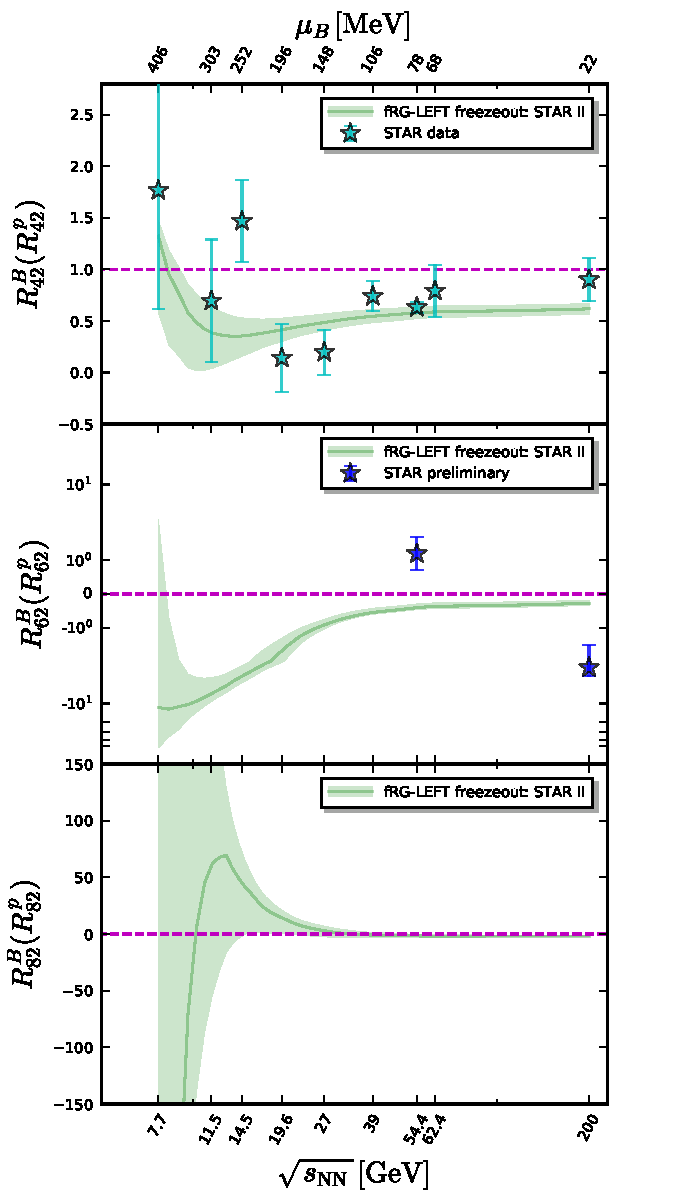
\includegraphics[width=0.45\textwidth]{Rm2-sqrtS2}
\caption{Baryon number fluctuations $R^{B}_{42}$ (top), $R^{B}_{62}$ (middle), and $R^{B}_{82}$ (bottom) as functions of the collision energy, calculated in LEFT within the fRG approach with the freeze-out parameters from STAR experiment \cite{Adamczyk:2017iwn}, where the parametrization of STAR freeze-out data is based on only the four data points in the middle region ($100\,\mathrm{MeV}\lesssim\mu_B\lesssim 300\,\mathrm{MeV}$) as shown in \Fig{fig:phasediagram}, and is designated as freezeout: STAR II. Experimental data of cumulants from the STAR collaboration are also shown for comparison, where $R^{p}_{42}$ (top) are the kurtosis of the net-proton distributions measured in Au+Au central (0-5\%) collisions \cite{Adam:2020unf}, and $R^{p}_{62}$ (middle) is the preliminary result on the six-order cumulant of the net-proton distribution at $\sqrt{s_{\mathrm{NN}}}$=200 GeV and 54.4 GeV with centrality 0-40\% \cite{Nonaka:2020crv,Pandav:2020uzx}. The horizontal dashed lines indicate positions of unity for $R^{B}_{42}$($R^{p}_{42}$), zeros for $R^{B}_{62}$($R^{p}_{62}$) and $R^{B}_{82}$.}\label{fig:Rm2-sqrtS2}\vspace{-0.5cm}
\end{figure}
%%%%%%%%%%%%%%%%%%%%%%%%%%%%%
%

In the following we would like to confront theoretical predictions on the baryon number fluctuations with experimental measurement. Frankly speaking, a direct comparison between the theory and experiment is a challenging task, or even impossible within the setup in this work. This is due to the fact that experimental data are affected by many factors, e.g.,  acceptance of the detector such as the transverse momentum $p_T$ range, rapidity window and the centrality dependence \cite{Adamczyk:2013dal,Luo:2015ewa,Adam:2020unf,Nonaka:2020crv,Pandav:2020uzx}, cf. also \cite{Luo:2017faz,Adamczyk:2017iwn} for more details, volume fluctuations \cite{Luo:2013bmi}, global baryon number conservation \cite{Braun-Munzinger:2016yjz,Vovchenko:2020tsr}, resonance decays \cite{Nahrgang:2014fza}, etc. They constitute the non-critical contributions to fluctuation observables in experiments, and pinning down their contributions plays a pivotal role in identifying the critical signals in the BES experiment. Additionally, \colfab{due to critical slowing down, nonequilibrium effects become important in the vicinity of the CEP \cite{Berdnikov:1999ph}}, which necessitates a theoretical description of the dynamics of critical fluctuations. For more details about recent progress on the dynamics of critical fluctuations in QCD, see \cite{Bluhm:2020mpc} and references therein. \colfab{We emphasize, however, that the present results are well outside the critical region and therefore not subject to critical dynamics.}

In this work we will not take into account the non-critical and dynamical effects discussed above when the theoretical results are confronted with experiments, but rather assume that the measured cumulants of the net-proton multiplicity distribution at a given collision energy, with other collision parameters e.g., the centrality and rapidity range fixed, is in one-by-one correspondence to the calculated fluctuations in \Eq{eq:suscept} with one value of $T$ or $\mu_B$. It is reasonable to attribute the values of $T$ and $\mu_B$ to be the ones when the chemical freeze-out occurs, viz. $T_{_{CF}}$ and ${\mu_B}_{_{CF}}$. Such an approach for the comparison is usually employed in fluctuation studies of equilibrium QCD matter within functional methods or lattice simulations \cite{Fu:2015amv,Isserstedt:2019pgx,Bazavov:2020bjn}. Note, however, that because of the reasons we have outlined above, results of comparison between the theory and experiment within this simplified approach should be taken with a grain of salt. In this work we adopt the freeze-out temperature and baryon chemical potential in \cite{Andronic:2017pug} and in STAR experiment \cite{Adamczyk:2017iwn}, which are shown in \Fig{fig:phasediagram} by the blue pentagons and red circles, respectively. They are both obtained from the analysis of hadron yields in the statistical hadron resonance gas model, see aforementioned references for more details. The freeze-out data in \cite{Andronic:2017pug} has also been parameterized as functions of the collision energy as follows
%
\begin{align}
   {\mu_B}_{_{CF}}&=\frac{a}{1+0.288\sqrt{s_{\mathrm{NN}}}},\label{eq:muBCFparatri}
\end{align}
%
with $a=1307.5$ MeV, and
%
\begin{align}
   T_{_{CF}}&=\frac{T^{lim}_{_{CF}}}{1+\exp\big(2.60-\ln(\sqrt{s_{\mathrm{NN}}})/0.45\big)},\label{eq:TCFparatri}
\end{align}
%
with $T^{lim}_{_{CF}}=158.4$ MeV. And this parametrization is depicted in \Fig{fig:phasediagram} by the blue dashed line. We use the same parametrization functions in Eqs. (\ref{eq:muBCFparatri}) and (\ref{eq:TCFparatri}) to fit the freeze-out data in STAR experiment, i.e., the red circle points in \Fig{fig:phasediagram}. Two parametrization curves are obtained: the red solid line and the green dotted one, where the former takes all the seven data points into account, while the latter only uses the four data points in the middle region ($100\,\mathrm{MeV}\lesssim\mu_B\lesssim 300\,\mathrm{MeV}$) for the fitting. The freeze-out curves of the red solid and green dotted lines in \Fig{fig:phasediagram} are labelled as freezeout: STAR I/II, respectively. The reason why we remove the first two data points in the low $\mu_B$ regime and the last one at $\mu_B\sim 400$ MeV in the parametrization of freezeout: STAR II, is due to the fact that the first two points are apparently higher than others and also a general consideration that the freeze-out curve in the plane of $T$-$\mu_B$ should be convex. One can see that, after these three data points are removed, the freeze-out line of STAR II moves down a bit to lower temperature in comparison to that of STAR I, which is more pronounced when $\mu_B\gtrsim 200$ MeV. 


















%In \Fig{fig:Rm2-sqrtS} we calculate baryon number fluctuations of different orders on the red solid and green dotted lines of \Fig{fig:phasediagram}, in order to investigate the influence of freeze-out parameters on the predicted collision-energy dependence. They are designated as freezeout: STAR I/II, respectively in \Fig{fig:phasediagram} and \Fig{fig:Rm2-sqrtS}. Furthermore, we also use the freeze-out data in \cite{Andronic:2017pug} through direct interpolation, and relevant results are shown in \Fig{fig:phasediagram} by the gray squares. 

%In this work we adopt the commonly used freeze-out temperature and baryon chemical potential in \cite{Andronic:2017pug}, which are obtained from the analysis of hadron yields in a hadron resonance gas model, as shown by the blue points in \Fig{fig:phasediagram}. Relevant freeze-out data have also been parameterized \cite{Andronic:2017pug} and, e.g., the dependence of freeze-out chemical potential on the collision energy is given by
%
%\begin{align}
%   {\mu_B}_{_{CF}}&=\frac{a}{1+0.288\sqrt{s_{\mathrm{NN}}}},\label{}
%\end{align}
%
%with $a=1307.5$ MeV, which is used in this work to determine ${\mu_B}_{_{CF}}$ for every $\sqrt{s_{\mathrm{NN}}}$. For the freeze-out temperature, we adopt two approaches. One is to use directly the parameterized chemical freeze-out temperature, which reads
%
%\begin{align}
%   T_{_{CF}}&=\frac{ T^{lim}_{_{CF}}}{1+\exp\big(2.60-\ln(\sqrt{s_{\mathrm{NN}}})/0.45\big)},\label{eq:TCFparatri}
%\end{align}
%
%and the relevant result as a function of ${\mu_B}_{_{CF}}$ is shown by the red dashed line in \Fig{fig:phasediagram}, and those corresponding to different collision energy are shown by red circles. The freeze-out temperature determined in \Eq{eq:TCFparatri} is denoted as the freeze-out: I in this work. Moreover, we also use another approach to determine the freeze-out temperature for different values of $\sqrt{s_{\mathrm{NN}}}$, to wit, interpolating it among the blue points in \Fig{fig:phasediagram}, and the relevant results are shown by the gray squares, which is denoted as freeze-out: II in the following. Freeze-out temperature for freeze-out: I and freeze-out: II, as well as the freeze-out baryon chemical potential, with different center-of-mass energy per nucleon pair $\sqrt{s_{\mathrm{NN}}}$ are presented in \Tab{tab:freeze-out-para}. One can see that the difference of freeze-out temperature between freeze-out: I and freeze-out: II is as large as $\sim 5$ MeV, which is large enough to allow us to study the error of calculations stemming from the determination of $T_{_{CF}}$.

%As we will see below, the theoretically predicted dependence of baryon number fluctuations on the collision energy is less sensitive to ${\mu_B}_{_{CF}}$ in contradistinction to $T_{_{CF}}$. Hence we adopt a phenomenological relation between the freeze-out chemical potential and the center-of-mass energy per nucleon pair $\sqrt{s_{\mathrm{NN}}}$, which reads
%
%\begin{align}
%   {\mu_B}_{_{CF}}&=\frac{a}{1+0.288\sqrt{s_{\mathrm{NN}}}},\label{}
%\end{align}
%
%with $a=1307.5$ MeV, which is obtained from the analysis of hadron yields in a hadron resonance gas model \cite{Andronic:2017pug}. As for the freeze-out temperature, we would like to employ the experimentally measured kurtosis of the net-proton multiplicity distribution to determine $T_{_{CF}}$. This is motivated by the consideration as follows. On the one hand, we are more interested in, and thus focus on the hyper-order fluctuations in this work, and more discussions about fluctuations and correlations of lower-orders could be found in, e.g., \cite{Fu:2015naa,Fu:2015amv,Fu:2016tey,Fu:2018swz}. On the other hand, it is interesting and valuable in itself to know that, if a theory can produce the experimental data of the fourth-order fluctuations, what would it predict for the hyper-order fluctuations. Hence, we use the relation which reads
%
%\begin{align}
%   R^B_{42}(T_{_{CF}})&=R^p_{42}(T_{_{CF}}),\label{eq:TCFR42}
%\end{align}
%
%to determine $T_{_{CF}}$ whenever it is possible, where the term $R^{B}_{42}$ on the l.h.s. is calculated from the theory and that on the right is the kurtosis of the net-proton distribution measured in the experiment, see the top panel of \Fig{fig:Rm2-sqrtS}. This approach works well except for three values of the collision energy, i.e., $\sqrt{s_{\mathrm{NN}}}$=27 GeV, 19.6 GeV, and 14.5 GeV, since their relevant experimental data are beyond the range of the corresponding theoretical predictions during the chiral phase transition regime, as shown in the left panel of \Fig{fig:R42R62R82-T-muB0to400}. Thus, we adopt the pseudocritical temperature of the chiral crossover for these three values of collision energy instead, which is extracted from the infection point of the chiral order parameter, i.e., the expectation value of the sigma field $\langle \sigma \rangle$ as a function of $T$ with $\mu_B$ fixed. And the relevant theoretical results of $R^B_{42}$ for these three values of $\sqrt{s_{\mathrm{NN}}}$ are also presented in the top panel of \Fig{fig:Rm2-sqrtS}, and one can see that for $\sqrt{s_{\mathrm{NN}}}$=27 GeV, 19.6 GeV, the theoretical results are not far from the experimental data, which is in sharp contrast to the case of $\sqrt{s_{\mathrm{NN}}}$=14.5 GeV. Finally, we present values of $T_{_{CF}}$ and ${\mu_B}_{_{CF}}$ for different collision energies in \Tab{tab:freeze-out-para}, which underlie the predictions for the hyper-order baryon number fluctuations in \Fig{fig:Rm2-sqrtS}.

In \Fig{fig:Rm2-sqrtS} we show the dependence of baryon number fluctuations $R^{B}_{42}$, $R^{B}_{62}$, and $R^{B}_{82}$ on the center-of-mass collision energy, which is calculated in the LEFT within the fRG approach with the freeze-out parameters from Andronic {\it et al.} \cite{Andronic:2017pug} and the freeze-out line of STAR I. Note that the freeze-out data from Andronic {\it et al.} are used through direct interpolation, and the resulting results are shown in \Fig{fig:phasediagram} by the gray squares. The theoretical results are also confronted with experimental measurement of cumulants of the net-proton distributions in the beam energy scan experiments from the STAR collaboration. The kurtosis of the net-proton distributions $R^{p}_{42}$ are measured in Au+Au collisions with centrality 0-5\%, transverse momentum range $0.4< p_T\,(\mathrm{GeV}/c)\,<2.0$, and rapidity $|y|<0.5$, cf. \cite{Adam:2020unf} for more details. Moreover, preliminary results for the six-order cumulant of the net-proton distribution $R^{p}_{62}$ are also presented in the middle plot of \Fig{fig:Rm2-sqrtS}, which are obtained at two values of the collision energy, i.e., $\sqrt{s_{NN}}$=200 GeV and 54.4 GeV with centrality 0-40\% \cite{Nonaka:2020crv,Pandav:2020uzx}. In \Fig{fig:Rm2-sqrtS2} we show a similar calculation but with the freeze-out line of STAR II, and compare it with the experiment measurement as well.

As shown in \Fig{fig:Rm2-sqrtS} as well as \Fig{fig:Rm2-sqrtS2}, the theoretical result of the fourth-order fluctuations calculated in the fRG-LEFT approach with the freeze-out data from Andronic {\it et al.}, as shown by the gray squares and band, is in qualitative agreement with the experimental measurement of the kurtosis of net-proton distributions.  In particular, a nonmonotonic behavior in the low collision energy regime, below $\sim 20$ GeV, is found in the fRG calculation. The nonmonotonic behavior is also found in the results with the freezeout parametrizations STAR I and STAR II. The nonmonotonic behavior from STAR I is significantly weaker than the others because the freeze-out temperature of STAR I is larger than the two others, in particular in the region of high $\mu_B$, as shown in \Fig{fig:phasediagram}. 
\colfab{This shows that even small variations in the freeze-out temperature have a substantial effect on the fluctuations. The underlying reason is that the freezout happens in or close to the crossover region, where the fluctuations vary significantly, see \Fig{fig:R42R62R82-T-muB0to400}.}

\colfab{
It is important to emphasize that the strong nonmonotonic behavior of our results for $R^{B}_{42}$ at small beam-energies in the top panel of \Fig{fig:Rm2-sqrtS} has nothing to do with critical physics. In our model, the CEP is at significantly larger $\mu_B$ [do we have a number?], and it is well established that the critical region is only very small, see e.g.\ \cite{Schaefer:2006ds}. This is a crucial point since a nonmonotonic behavior, e.g., of $R^{B}_{42}$ as a function of $\sqrt{s_{NN}}$ has been proposed as an experimental signature of a CEP \cite{Stephanov:1999zu, Stephanov:2011pb}. However, these works only show that critical physics is sufficient for nonmonotonic behavior. Our results unequivocally demonstrate that critical behavior not \emph{necessarily} leads to nonmonotonic behavior, it also occurs at finite $\mu_B$ far away from a CEP. In the present case, it is a result of two effects. First, correlations are enhanced since the chiral crossover becomes sharper with increasing $\mu_B$. This leads to stronger nonmonotonic behavior of $R^{B}_{42}$ as a function of $T$ (see \Fig{fig:R42R62R82-T-muB0to400}.). Second, the freeze-out temperature is shifted away from the pseudocritical temperature towards small beam-energies, thereby probing different regimes of the cumulants.
}

%Consequently, the strong nonmonotonic behavior of $R^{p}_{42}$ in the low collision energy regime observed in the experiment indicates that, firstly the critical region near the CEP is being approached in the low collision energy region, or if there is no CEP, the value of $R^{p}_{42}$ can not exceed 1, conversely the experiment finds the central value of $R^{p}_{42}$ between 1.5 and 2 at $\sqrt{s_{NN}}$=7.7 GeV, though the error is still large there; secondly, the freeze-out temperature in the high-$\mu_B$ region should be relatively lower, otherwise if it was as high as the STAR I, the kurtosis of baryon number distribution should go down monotonously like the red circles in the top panel of \Fig{fig:Rm2-sqrtS}, rather than bump up with the decrease of collision energy. As a matter of fact, the freeze-out temperature is beginning to be smaller than the pseudo-critical temperature of the chiral crossover, when $\mu_B$ is increased beyond $300\sim400$ MeV, as shown in Fig.1 in \cite{Fu:2019hdw}.

\colfab{
Moreover, the nonmonotonic behavior is also observed in the sixth-order and eighth-order baryon number fluctuations as functions of the collision energy, as shown in the center and bottom panel of \Fig{fig:Rm2-sqrtS} and \Fig{fig:Rm2-sqrtS2}. 
\colfab{The discussion of the previous paragraph clearly also applies here.}
However, it should be noted that the error of our results increases significantly in the low energy region. These errors include the systematic error of the fRG-LEFT approach, which stem from the uncertainty in the matching of the in-medium scales of the LEFT and QCD, encoded in the coefficients $c_{_{T}}$ and $c_{\mu}$ in \Eq{eq:rescale}.% Furthermore, baryon number fluctuations calculated with the STAR freeze-out parameters also take the errors of freeze-out data, i.e., the errors of the red circles in \Fig{fig:phasediagram}, into account, resulting in an overall larger error for the freezout parametrization STAR I and STAR II (red and green in \Fig{fig:Rm2-sqrtS}) as compared to Andronic {\it et al.} (gray in \Fig{fig:Rm2-sqrtS}). 
For $\sqrt{s_{NN}}$=200 GeV and 54.4 GeV we can compare our results for $R^{B}_{62}$ to preliminary STAR data \cite{Nonaka:2020crv,Pandav:2020uzx}. As opposed to $R^{B}_{42}$, we find large deviations between our and the experimental results. At the highest beam energy, $\sqrt{s_{NN}}$=200 GeV, we at least agree qualitatively in that $R^{B}_{42}$ is negative.
}



%Comparing the red bands with the gray ones, one finds that errors of the freeze-out temperature lead to significant errors of baryon number fluctuations predicted in the low collision energy regime, and hence a determination of freeze-out temperature with high precision in the region is highly required in the future.
 

%As we have discussed above, the overall agreement between the theory and experiment for the fourth-order fluctuations is reasonable and natural, since the experimental data of $R^{p}_{42}$ have been used to fix the freeze-out temperature, except for few values of the collision energy. With the setting-up in hand, one can use the fRG-LEFT approach to predict the dependence of hyper-order fluctuations on the collision energy, as shown in the middle and bottom panels of \Fig{fig:Rm2-sqrtS}. A crude estimate for the systematic error of theoretical calculation is indicated by the red bands in \Fig{fig:Rm2-sqrtS}, which directly results from errors of the scale matching coefficients $c_{_{T}}$ and $c_{\mu}$ in \Eq{eq:rescale}. We find that, with the decrease of collision energy, $R^{B}_{62}$ in LEFT goes down crossing the zero line, and finally bumps up at the last collision energy. It should, however, be noticed that the relevant error for $R^{B}_{62}$ increases rapidly when the collision energy is below $\sim 20$ GeV.

%The coefficient $c_{_{T}}$ in \Eq{eq:rescale} is fixed through the relative values of the pseudocritical temperature at $\mu_B=0$ in the LEFT and QCD, i.e., $c_{_{T}}=T_{c_{LEFT}}/T_c$, where $T_c=156$ MeV is employed for QCD from the lattice simulations. Hence, determination of $T_{c_{LEFT}}$ in the LEFT plays a key role in fixing the coefficient $c_{_{T}}$. Unfortunately, the chiral phase transition with the temperature at $\mu_B=0$ is not an exact phase transition, but rather a continuous crossover, due to a finite current quark mass. Accordingly, different observables might result in nonidentical $T_{c_{LEFT}}$. Since we are concerned with the baryon number fluctuations in this work, the kurtosis of the baryon number distribution, i.e., $\kappa \sigma^2=\chi_4^{B}/\chi_2^{B}$, is used to fix $T_{c_{LEFT}}$ as follows. In the left panel of \Fig{fig:R42R62R82-T-muB0}, $\chi_4^{B}/\chi_2^{B}$ is shown as a function of the temperature in unit of $T_c$ with vanishing baryon chemical potential, and result of the LEFT within fRG is compared with that of lattice QCD. It is found that the LEFT within fRG gives the best description of $\kappa \sigma^2$ in comparison to the lattice results with $T_{c_{LEFT}}=195$ MeV, which yields  
%\begin{align}
%  c_{_{T}}&=T_{c_{LEFT}}/T_c=1.25\,.\label{eq:cT}
%\end{align}
%From now on unless explicitly specified, values of temperature in the following, e.g., in legends of figures, are always referred to $T$, and the relevant $T_{_{LEFT}}$ in the LEFT could be inferred from Eqs. (\ref{eq:rescale}) and (\ref{eq:cT}).


%%%%%%%%%%%%%%%%%%%%%%%%%%%%%%%%%%%%%%%%%%%%%%%%%%%%%%%%%%%
%%%%%%%%%%%%%%%%%%%%%%%%%%%%%%%%%%%%%%%%%%%%%%%%%%%%%%%%%%%

\section{summary and conclusions}
\label{sec:summary}

In this work we have studied the baryon number fluctuations in the LEFT within the fRG approach, putting emphasis on the hyper-order ones. The order of baryon number fluctuations has been computed up to the $10^{\mathrm{th}}$ order for the first time beyond mean-field. In our calculations, quantum, thermal and density fluctuations are successively encoded through the evolution of flow equations. Moreover, nontrivial dispersion relation for the quark and meson fields, momentum scale dependence of the quark-meson scattering, and fluctuations of Polyakov loop are also taken into account in this work.

The scale between the LEFT and QCD is matched via a comparison of the temperature dependence of $R^{B}_{42}=\chi^{B}_{4}/\chi^{B}_{2}$ at vanishing $\mu_B$ between the LEFT and lattice results, as well as a comparison of the curvature of phase boundary. Accordingly, it allows us to employ the LEFT within the fRG approach to make predictions for the $\mu_B$-dependence of $R^{B}_{42}$, and the hyper-order baryon number fluctuations at finite temperature and density. In turn, relevant predictions of LEFT are compared with results of lattice QCD simulations. We find that the $T$- and $\mu_B$-dependence of hyper-order baryon number fluctuations, $\mu_B$-dependence of $R^{B}_{42}$ obtained in the fRG-LEFT approach, are in quantitative accordance with the lattice results by the Wuppertal-Budapest collaboration within errors. There is still a sizable quantitative deviation in comparison to relevant results by the HotQCD collaboration, but a qualitative consistency is observed.

Furthermore, by employing the commonly used chemical freeze-out temperature and baryon chemical potential from Andronic {\it et al.} \cite{Andronic:2017pug} and STAR experiment \cite{Adamczyk:2017iwn}, we obtain baryon number fluctuations $R^{B}_{42}$, $R^{B}_{62}$, and $R^{B}_{82}$ as functions of the collision energy, which are compared with experimental measurements of the kurtosis and sixth-order cumulants of the net-proton distributions from the STAR collaboration. Remarkably, the dependence of the fourth-order baryon number fluctuation $R^{B}_{42}$ on the collision energy obtained in the fRG-LEFT approach, is qualitative consistent with the experimental measured dependence of the kurtosis of net-proton distributions on the collision energy for central collisions. And a nonmonotonic behavior of $R^{B}_{42}$ as a function of $\sqrt{s_{\mathrm{NN}}}$ is found in the fRG calculation. It should, however, be cautioned that errors of $R^{B}_{42}$ and $R^{B}_{62}$ increase significantly in the low collision energy region. And when the order of baryon number fluctuations is increased up to the $8^{\mathrm{th}}$, the theoretical calculation with current setup is losing its capability of making predictions, as a consequence of the significant errors of $R^{B}_{82}$ for large range of collision energy. Apparently, in order to improve on the computation in this work in the future, and decrease the errors of calculated baryon number fluctuations, especially in the low collision energy regime, on the one hand, the systematic errors of theoretical calculations should be reduced, and on the other hand, chemical freeze-out data with high precision are highly required.



%%%%%%%%%%%%%%%%%%%%%%%%%%%%%%%%%%%%%%%%%%%%%%%%%%%%%%%%%%%
%%%%%%%%%%%%%%%%%%%%%%%%%%%%%%%%%%%%%%%%%%%%%%%%%%%%%%%%%%%

\begin{acknowledgments}

We thank Nu Xu for discussions. The work was supported by the National Natural Science Foundation of China under Contracts Nos. 11775041.

......

\end{acknowledgments}

%%%%%%%%%%%%%%%%%%%%%%%%%%%%%%%%%%%%%%%%%%%%%%%%%%%%%%%%%%%%%
%%%%%%%%%%%%%%%%%%%%%%%%%%%%%%%%%%%%%%%%%%%%%%%%%%%%%%%%%%%%%

\appendix

\section{Glue potential}
\label{app:gluepot}

As we have discussed in \sec{sec:FRG}, the dynamics of the glue sector in QCD is partly imprinted in the glue potential $V_{\mathrm{glue},k}(A_0)$, cf. \Eq{eq:Vtotal}, when the RG scale is in the regime of LEFT. We neglect the scale dependence of the glue potential in this work, and assume
%
\begin{align}
   V_\mathrm{glue}(L,\bar{L})&=V_{\mathrm{glue},k=0}(A_0)=T^4 \bar V_\mathrm{glue}(L,\bar{L}),\label{}
\end{align}
%
where we have introduced a dimensionless glue potential $\bar V_\mathrm{glue}$, and its dependence on the temporal background $A_0$ field is realized via the traced Polyakov loop $L$ and its conjugate $\bar{L}$, which reads
%
\begin{align}
  L(\bm{x})&=\frac{1}{N_c} \left\langle \Tr\, {\cal P}(\bm x)\right\rangle\,,\quad  \bar L (\bm{x})=\frac{1}{N_c} \langle \Tr\,{\cal P}^{\dagger}(\bm x)\rangle \,,\label{eq:Lloop}
\end{align}
%
with 
%
\begin{align}
  {\cal P}(\bm x)&=\mathcal{P}\exp\Big(ig\int_0^{\beta}d\tau \hat A_0(\bm{x},\tau)\Big)\,, \label{eq:Ploop}
\end{align}
%
where $\mathcal{P}$ on the r.h.s. is the path ordering operator. In this work we adopt the parametrization of the glue potential in \cite{Lo:2013hla}, which reads
%
\begin{align}
  V_\text{glue}(L,\bar{L})=& -\frac{a(T)}{2} \bar L L + b(T)\ln M_H(L,\bar{L})\nonumber \\[2ex]
  &+ \frac{c(T)}{2} (L^3+\bar L^3) + d(T) (\bar{L} L)^2\,,
                             \label{eq:polpot}
\end{align}
%
with the $\mathrm{SU}(N_c)$ Haar measure
%
\begin{align}
  M_H (L, \bar{L})&= 1 -6 \bar{L}L + 4 (L^3+\bar{L}^3) - 3  (\bar{L}L)^2\,.
\end{align}
%
Note that the parametrization of glue potential in \Eq{eq:polpot}, as well as determination of relevant parameters in \Tab{tab:gluepotCoeffs}, is done based on lattice results of  $\mathrm{SU}(3)$ Yang-Mills theory at finite temperature, where not only the expectation value of the Polyakov loop and pressure, but also quadratic fluctuations of the Polyakov loop are taken into account \cite{Lo:2013hla}. The coefficients in \Eq{eq:polpot} are dependent on the temperature, which reads
%
\begin{align}
  x(T) &= \frac{x_1 + x_2/(t_r+1) + x_3/(t_r+1)^2}{1 + x_4/(t_r+1) + x_5/(t_r+1)^2}\,,\label{eq:xT}
\end{align}
%
for $x\in \{a, c, d\}$, and 
%
\begin{align}
  b(T) &=b_1 (t_r+1)^{-b_4}\left (1 -e^{b_2/(t_r+1)^{b_3}} \right)\,,\label{eq:bT}
\end{align}
%
with the reduced temperature $t_r=(T-T_c)/T_c$, and the parameters in \Eq{eq:xT} and \Eq{eq:bT} have been fixed in \cite{Lo:2013hla} and their values are also collected in \Tab{tab:gluepotCoeffs} for convenience.

Though the parametrization of the glue potential in \Eq{eq:polpot} is based on results of the Yang-Mills theory, it has found that the unquenching effect in QCD is well captured, once a linear rescaling of the reduced temperature is made from the pure gauge theory to QCD \cite{Pawlowski:2010ht, Haas:2013qwp, Herbst:2013ufa}, as follows
%
\begin{align}
  (t_r)_{\text{\tiny{YM}}}&\rightarrow \alpha\,(t_r)_{\text{\tiny{glue}}}\,,\label{}
\end{align}
%
with
%
\begin{align}
  (t_r)_{\text{\tiny{glue}}}&=
    (T-T_c^\text{\tiny{glue}})/T_c^\text{\tiny{glue}}\,,\label{}
\end{align}
%
where we have used $\alpha=0.7$ and $T_c^\text{\tiny{glue}}$=216 MeV (in unit of physical temperature via \Eq{eq:rescale}) in this work.


%
 %%%%%%%%%%%
\begin{table}[tb!]
  \begin{center}
    \begin{tabular}{|c||c|c|c|c|c|}
    \hline & & & & &  \\[-2ex]
    \hline & & & & & \\[-1ex]
     & 1 & 2 & 3 & 4 & 5 \\[1ex]
    \hline & & & & &  \\[-2ex]
    $a_i$ &-44.14& 151.4 & -90.0677 &2.77173 &3.56403 \\[1ex]
    \hline & & & & &  \\[-2ex]
    $b_i$ &-0.32665 &-82.9823 &3.0 &5.85559  &              \\[1ex]
    \hline & & & & &  \\[-2ex]
    $c_i$ &-50.7961 &114.038 &-89.4596 &3.08718 &6.72812 \\[1ex]
    \hline & & & & &  \\[-2ex]
    $d_i$ & 27.0885 &-56.0859 &71.2225 &2.9715 &6.61433 \\[1ex]
    \hline
    \end{tabular}
    \caption{Values of the parameters in \eq{eq:xT} and \eq{eq:bT} for the glue potential.}
    \label{tab:gluepotCoeffs}
  \end{center}\vspace{-0.5cm}
\end{table}
%%%%%%%%%%%%
%

%%%%%%%%%%%%%%%%%%%%%%%%%%%%%%%%%%%%%%%%%%%%%%%%%%%%%%%%%%%%%
\section{Flow equations}
\label{app:flowV}

The flow equation for the effective potential of the matter sector is given in \Eq{eq:flowV}. In this work we use the Taylor expansion approach to solve this equation numerically. Expanding the potential around a $k$-dependent value $\kappa_k$, one arrives at 
%
\begin{align}
  V_{\mathrm{mat}, k}(\rho)&=\sum_{n=0}^{N_v}\frac{\lambda_{n,k}}{n!}(\rho-\kappa_k)^n\,, \label{eq:VTaylor}
\end{align}
%
with the expansion coefficients $\lambda_{n,k}$'s, where $N_v$ is the maximal order of Taylor expansion included in the numerical calculation. It is more convenient to rewrite \Eq{eq:VTaylor} by means of the renormalized variables, i.e.,
%
\begin{align}
  \bar V_{\mathrm{mat}, k}(\bar \rho)&=\sum_{n=0}^{N_v}\frac{\bar\lambda_{n,k}}{n!}(\bar \rho-\bar \kappa_k)^n\,,\label{eq:VbarTaylor}
\end{align}
%
with $\bar V_{\mathrm{mat}, k}(\bar \rho)=V_{\mathrm{mat}, k}(\rho)$, $\bar \rho=Z_{\phi,k} \rho$, $\bar \kappa_k=Z_{\phi,k}\kappa_k$, and $\bar \lambda_{n,k}=\lambda_{n,k}/(Z_{\phi,k})^n$. Inserting \Eq{eq:VbarTaylor} into the l.h.s. of \Eq{eq:flowV} leads us to
%
\begin{align}
  &\partial^n_{\bar \rho}\left(\partial_t\big|_{\rho} \bar V_{\mathrm{mat}, k}(\bar \rho)\right)\Big|_{\bar \rho=\bar \kappa_k}\nonumber\\[2ex]
=&(\partial_t -n\eta_{\phi,k})\bar{\lambda}_{n,k}-(\partial_t \bar \kappa_k+\eta_{\phi,k}\bar \kappa_k)\bar \lambda_{n+1,k}\,.\label{eq:drhoV}
\end{align}
%

In our calculation, the expansion point $\kappa_k$ in \Eq{eq:VTaylor} or $\bar \kappa_k$ in \Eq{eq:VbarTaylor} is chosen such that it is the minimum of the effective action in \Eq{eq:action}, which yields the equation of motion as follows
%
\begin{align}
  \frac{\partial}{\partial \bar \rho}\Big(\bar V_{\mathrm{mat}, k}(\bar \rho)-\bar c_k
  \bar \sigma \Big)\bigg \vert_{\bar\rho=\bar \kappa_k}&=0\,, \label{eq:Vstat}
\end{align}
%
with $ \bar \sigma=Z_{\phi,k}^{1/2} \sigma$ and $\bar c_k=Z_{\phi,k}^{-1/2} c$, where $c$ is independent of the IR cutoff $k$. This expansion is usually called the physical running expansion, since the bare expansion point $\kappa_k$ is $k$-dependent as mentioned above. In contrast, another commonly used expansion approach is the fixed-point expansion, and as its name suggests, in this approach the bare expansion point is $k$-independent. For more discussions about these two different expansion approaches, and their advantages and disadvantages in the application of fRG calculations, see e.g.,  \cite{Pawlowski:2014zaa,Braun:2014ata, Fu:2015naa, Rennecke:2016tkm,Yin:2019ebz}. Combination of \Eq{eq:drhoV} and \Eq{eq:Vstat} leaves us with the flow equation for the expansion point, which reads
%
\begin{align}
  \partial_t \bar \kappa_k&=-\frac{\bar c_k^2}{\bar{\lambda}_{1,k}^3+\bar c_k^2\bar{\lambda}_{2,k}}\bigg[\partial_{\bar \rho}\left(\partial_t\big|_{\rho} \bar V_{\mathrm{mat}, k}(\bar \rho)\right)\Big|_{\bar \rho=\bar \kappa_k}\nonumber \\[2ex]
          &+\eta_{\phi,k}\left(\frac{\bar{\lambda}_{1,k}}{2}+\bar\kappa_k\bar{\lambda}_{2,k}\right)\bigg]\,.\label{eq:flowkappa}
\end{align}
%

The meson anomalous dimension in \Eq{eq:etaphi} reads
%
\begin{align}
  \eta_{\phi,k}&=\frac{1}{6\pi^2}\Bigg\{\frac{4}{k^2} \bar{\kappa}_k(\bar{V}''_k(\bar{\kappa}_k))^2\mathcal{BB}_{(2,2)}(\tilde{m}^{2}_{\pi,k},\tilde{m}^{2}_{\sigma,k};T)\nonumber\\[2ex]
&+N_c\bar{h}^{2}_{k}\bigg[\mathcal{F}_{(2)}(\tilde{m}^{2}_{q,k};T,\mu)(2\eta_{q,k}-3)\nonumber\\[2ex]
&-4(\eta_{q,k}-2)\mathcal{F}_{(3)}(\tilde{m}^2_{q,k};T,\mu)\bigg]\Bigg\}\,, \label{eq:etaphi2}  
\end{align} 
%
The quark anomalous dimension in \Eq{eq:etapsi} reads
\begin{align}
\eta_{q,k}=&\frac{1}{24\pi^2N_f}(4-\eta_{\phi,k})\bar{h}^{2}_{k}\nonumber\\[2ex]
&\times\bigg\{ (N^{2}_{f}-1)\mathcal{FB}_{(1,2)}(\tilde{m}^{2}_{q,k},\tilde{m}^{2}_{\pi,k};T,\mu,p_{0,ex})\nonumber\\[2ex]
&+\mathcal{FB}_{(1,2)}(\tilde{m}^{2}_{q,k},\tilde{m}^{2}_{\sigma,k};T,\mu,p_{0,ex})\bigg\}\,, \label{eq:etapsi2}
\end{align} 
where in the threshold function $\mathcal{FB}$'s we have employed $p_{0,ex}=\pi T$ for the finite temperature sector and $p_{0,ex}=\pi T\exp\{-k/(\pi T)\}$ for the vacuum sector. The modification for the vacuum sector is necessitated in order to suppress the artefact of temperature dependence of thermodynamics in the low temperature region \cite{Fu:2015naa}, which can be resolved by means of frequency summation of the quark external leg \cite{Fu:2016tey}. The flow of the Yukawa coupling in \Eq{eq:dth} is given by
\begin{align}
  \partial_t&\bar{h}_k=\left(\frac{1}{2}\eta_{\phi,k}+\eta_{q,k}\right)\bar{h}_k(\bar{\rho})\nonumber\\[2ex]
&+\frac{\bar{h}^3_k}{4\pi^2N_f}\bigg[L^{(4)}_{(1,1)}(\tilde{m}^{2}_{q,k},\tilde{m}^{2}_{\sigma,k},\eta_{q,k},\eta_{\phi,k};T,\mu,p_{0,ex})\nonumber\\[2ex]
&-(N^{2}_{f}-1)L^{(4)}_{(1,1)}(\tilde{m}^{2}_{q,k},\tilde{m}^{2}_{\pi,k},\eta_{q,k},\eta_{\phi,k};T,\mu,p_{0,ex})\bigg]\,.\label{eq:dth2}  
\end{align} 
Note that explicit expressions of all the threshold functions mentioned above, such as $\mathcal{BB}$, $\mathcal{F}$'s, $\mathcal{FB}$'s, and $L$ can be found in e.g., \cite{Fu:2019hdw,Yin:2019ebz}.

To summarize, flow equations (\ref{eq:flowV}), (\ref{eq:drhoV}), (\ref{eq:flowkappa}), (\ref{eq:dth2}) supplemented with \Eq{eq:etaphi2} and \Eq{eq:etapsi2} constitute a closed set of ordinary differential equations, which is evolved from the UV cutoff $k=\Lambda$ to the IR limit $k=0$. The parameters of LEFT are given by initial values of the flow equations. To be specific, the effective potential of the matter sector at the UV cutoff reads
\begin{align}
  V_{\mathrm{mat}, k=\Lambda}(\rho)=\frac{\lambda_{k=\Lambda}}{2}\rho^2+\nu_{k=\Lambda}\rho\,,
\end{align}
with $\lambda_{k=\Lambda}=11$ and $\nu_{k=\Lambda}=(0.830\,\mathrm{GeV})^2$. In addition, the initial value of the Yukawa coupling is $h_{k=\Lambda}=10.18$, and the explicit chiral symmetry breaking parameter is $c=2.82\times 10^{-3}\,\mathrm{GeV}^3$. These parameters are fixed by fitting the hadronic observables in vacuum, i.e., $f_\pi=92\,\mathrm{MeV}$, $m_q=306\,\mathrm{MeV}$, $m_\pi=136\,\mathrm{MeV}$,and $m_\sigma=483\,\mathrm{MeV}$.




%%%%%%%%%%%%%%%%%%%%%%%%%%%%%%%%%%%%%%%%%%%%%%%%%%%%%%%%%%%%%%%%
%%%%%%%%%%%%%%%%%%%%%%%%%%%%%%%%%%%%%%%%%%%%%%%%%%%%%%%%%%%%%%%%
% The \nocite command causes all entries in a bibliography to be
% printed out whether or not they are actually referenced in the
% text. This is appropriate for the sample file to show the different
% styles of references, but authors most likely will not want to use
% it.  \nocite{*}

%\bibliography{refspec}% Produces the bibliography via BibTeX.
\bibliography{ref-lib}% Produces the bibliography via BibTeX.


\end{document}
